%%
%%	AVISO IMPORTANTE
%%	Formato optimizado para el sistema operativo GNU/Linux 64 bits
%%	usar TexLive 2016 (o superior), http://www.ctan.org/tex-archive/systems/texlive/Images/
%%	usar TeXstudio 2.11, http://texstudio.sourceforge.net/

\documentclass[letterpaper,12pt]{thesisECFM}
\usepackage{macros}
\usepackage{verbatim}
%%	NO OLVIDE INCLUIR FUENTE DE LAS TABLAS Y FIGURAS

% Decomentar para anular recuadros en los hiperenlaces dentro del pdf
% \hypersetup{pdfborder={0 0 0}}

% Teoremas ---------------------------------------------------------
% estos ambientes son para teoremas, lemas, corolarios, otros
% si no los utiliza los puede obviar en su trabajo de graduación
\theoremstyle{plain}
\newtheorem{thm}{Teorema}[section]
\newtheorem{cor}{Corolario}[chapter]
\newtheorem{lem}{Lema}[chapter]
\newtheorem{prp}{Proposición}[chapter]

\theoremstyle{definition}
\newtheorem{exa}{Ejemplo}[chapter]
\newtheorem{defn}{Definición}[chapter]
\newtheorem{axm}{Axioma}[chapter]

\theoremstyle{remark}
\newtheorem{rem}{Nota}[chapter]

% Operadores y funciones -------------------------------------------
% Los siguientes son ejemplos de comandos definidos por el usuario
% puede borrarlos, únicamente están para mostrar cómo se construyen con LaTeX
\DeclareMathOperator{\Supp}{Supp}       \DeclareMathOperator{\vol}{Vol}%
\DeclareMathOperator{\Rz}{Re}           \DeclareMathOperator{\Iz}{Im}%

\newcommand{\R}{\mathbb{R}}             \newcommand{\Z}{\mathbb{Z}}%
\newcommand{\C}{\mathbb{C}}             \newcommand{\K}{\mathbb{K}}%
\newcommand{\N}{\mathbb{N}}             \newcommand{\Q}{\mathbb{Q}}%
\newcommand{\Af}{\mathfrak{A}}          \newcommand{\Bf}{\mathfrak{B}}%
\newcommand{\Cf}{\mathfrak{C}}          \newcommand{\Df}{\mathfrak{D}}%
\newcommand{\Ff}{\mathfrak{F}}          \newcommand{\Lf}{\mathfrak{L}}%
\newcommand{\Mf}{\mathfrak{M}}          \newcommand{\Sf}{\mathfrak{S}}%
\newcommand{\Hi}{\mathcal{H}}           \newcommand{\Ba}{\mathcal{B}}%
\newcommand{\nada}{\varnothing}         \newcommand{\To}{\longrightarrow}%
\newcommand{\RR}{[-\infty,+\infty]}     \newcommand{\df}{:=}%
\newcommand{\sani}{$\sigma$\nobreakdash-anillo}
\newcommand{\salg}{$\sigma$\nobreakdash-álgebra}
\newcommand{\ff}{f^{-1}}

\newcommand{\norm}[1]{\left\Vert#1\right\Vert}
\newcommand{\pnorm}[2]{\norm{#1}_{#2}}
\newcommand{\abs}[1]{\left\vert#1\right\vert}
\newcommand{\su}[2]{\left\{#1_{#2}\right\}}
\newcommand{\Su}[4]{\suce #1#2 _{#2=#3}^{#4}}
\newcommand{\union}[4]{\bigcup_{{#2}={#3}}^{#4} #1_{#2}}
\newcommand{\Union}[4]{\bigcup \limits_{{#2}={#3}}^{#4} #1_{#2}}
\newcommand{\inter}[4]{\bigcap_{{#2}={#3}}^{#4} #1_{#2}}
\newcommand{\Inter}[4]{\bigcap \limits_{{#2}={#3}}^{#4} #1_{#2}}

\newcommand{\pdual}[2]{\left<#1,#2\right>}
\newcommand{\bra}[1]{\left<#1\right\vert}
\newcommand{\ket}[1]{\left\vert#1\right>}
\newcommand{\braket}[2]{\left<#1\vert#2\right>}
\newcommand{\Braket}[2]{\left\vert#1\right>\! \left<#2\right\vert}
%%%%%%%%%%%%%%%%%%%%%%%%%%%%%%%%%%%%%%%%%%%%%%%%%%%%%%%%%%%%%%%%%%%%


% Cuerpo de la tesis -----------------------------------------------

\begin{document}
\begin{comment}
%% Datos generales del trabajo de graduación
\datosThesis%
{2}%						% física 1; matemática 2
{TEORÍA DE NUDOS Y SUS APLICACIONES}%		% Título del trabajo de graduación
{Billy Othmaro}%			% autor
{Quevedo Carranza }%			% asesor
{Julio de 2017}		% mes y año de la orden de impresión
{2}							% femenino 1; masculino 2

%% Datos generales del examen general privado
\examenPrivado%
{M.Sc. Edgar Anibal Cifuentes Anléu}%	% director ECFM
{Ing. José Rodolfo Samayoa Dardón}%		% secretario académico
{Perengano}%		% examinador 1
{Zutano}%		% examinador 2
{Fulano 2}%		% examinador 3

{\onehalfspacing	% interlineado 1 1/2

\OrdenImpresion{ordenImpresion}		% incluye orden de impresión, guardada en pdf

\Agrade{agradecimientos}			% Agradecimientos

\Dedica{dedicatoria}				% Dedicatoria

\par}
 
\frontmatter    % --------------------------------------------------  Hojas preliminares

{\onehalfspacing	% interlineado 1 1/2

\tableofcontents    % Índice general vinculado

%%% \figurasYtablas{ lista_figuras }{ lista_tablas }; con valor 1 se incluye la lista,
%%% cualquier otro valor no la genera
\figurasYtablas{1}{1}

%%% INCLUYA LA SIMBOLOGÍA NECESARIA EN ESTE APARTADO
%%% NO CAMBIAR LA DEFINICIÓN DE LA TABLA LARGA


\chapter{LISTA DE SÍMBOLOS}

\begin{longtable}{@{}l@{\extracolsep{\fill}} p{4.75in} @{}}  %%%	NO CAMBIAR ESTA LÍNEA
  \textsf{Símbolo} & \textsf{Significado}\\[12pt]
  \endhead
  $:=$ & es definido por\\
  $\cong$ & es isomorfo a\\
  $\Leftrightarrow$ & si y sólo si\\
  $\varnothing$ & conjunto vacío\\
  $E^c$ & complemento de $E$\\
  $\varsubsetneq$ & estrictamente contenido\\
  $E\setminus F$ & diferencia entre $E$ y $F$\\
  $E\Delta F$ & diferencia simétrica entre $E$ y
  $F$\\
  $\mathcal{P} (X)$ & conjunto potencia de $X$\\
  $\chi_E$ & función característica de $E$\\
  $E_n\!\!\uparrow$ & $E_n$ es una sucesión
  creciente\\
  $\mathfrak{L}$ & \salg{} de los conjuntos
  Lebesgue"=medibles\\
  $\mathscr{S}$ & espacio muestral\\
  $\mathfrak{A}$ & \salg{} de eventos\\
  $(\mathscr{S},\mathfrak{A},P)$ & espacio de
  probabilidad\\
  $\mathscr{D}$ & espacio de las funciones de
  prueba\\
  $\mathscr{D}'$ & espacio de las distribuciones\\
  $\delta_0$ & medida de Dirac, función $\delta$ de Dirac o
  $\delta$-función\\
  $\Phi^{\times}$ & espacio antidual de $\Phi$\\
  $\Phi\subset \mathcal{H}\subset \Phi^{\times}$ &
  espacio de Hilbert equipado o tripleta de Gel'fand\\
  $\left\vert \psi \right>$ & vector \emph{ket}\\
  $\left< \psi \right\vert$ & funcional \emph{bra}\\
  $\left< \varphi \vert \psi \right>$ & \emph{braket}
\end{longtable}
  % Lista de símbolos

%%% Haga el diseño que más le guste
\chapter{OBJETIVOS}

\section*{General}
Escriba el objetivo general.


\section*{Específicos}
Enumere los objetivos específicos.
\begin{enumerate}
\item 
\item 
\end{enumerate}

      % Resumen y objetivos

%%% Haga el diseño que más le guste
\chapter{INTRODUCCIÓN}


      % Introducción
\end{comment}
\mainmatter     % --------------------------------------------------  Cuerpo del Trabajo de Graduación

\begin{comment}
\chapter{CONCEPTOS BÁSICOS DE TEORÍA DE NUDOS}
En el presente capítulo se presentan las definiciones y teoremas básicos en el estudio de la teoría de nudos. Se realizan las demostraciones que son cruciales para el contenido a desarrollar más adelante.

\section{Nudos y enlaces}
\subsection{Nudos}
Para el estudio matemático de lo que físicamente se comprende como un nudo se requiere plantear una definición matemática de nudo que concuerde con el modelo físico. Así la definición formal de un nudo es la siguiente:

\begin{defn}\label{dfcp1} El subconjunto $K\subset\mathbb{R}^3$ es un \textbf{nudo} si existe un homeomorfismo del círculo unitario $S^1$ en $\mathbb{R}^3$ cuya imagen es $K$.
\end{defn}

El ejemplo más simple de un nudo es la circunferencia $S^1$ vista en $\mathbb{R}^3$, este nudo es conocido como \textbf{no nudo} o \textbf{nudo trivial}, figura~\ref{fig:nudotrivial}, además otro ejemplo de un nudo simple es el \textbf{nudo trébol}, figura~\ref{fig:nudotrebol}.

\begin{figure}[ht]
	\centering
	\includegraphics[width=0.175\linewidth]{trebol}\\
	\caption[Nudo Trébol]{Nudo Trébol}
	\label{fig:nudotrebol}
\end{figure}

\begin{figure}[ht]
	\centering
	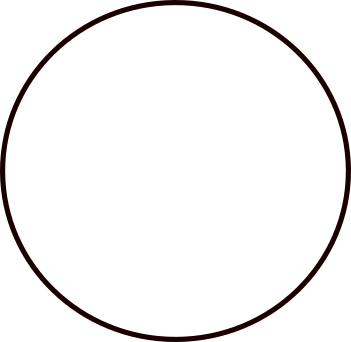
\includegraphics[width=0.175\linewidth]{Trivial}\\
	\caption[Nudo Trivial]{No Nudo o Nudo trivial}
	\label{fig:nudotrivial}
\end{figure}

El primer interrogante que surge al hablar sobre el nudo trivial y el nudo trébol es: ¿cómo saber que efectivamente estos dos nudos son distintos? Para resolver a esta pregunta primero se debe definir cuando dos nudos son el mismo nudo.

\begin{defn}\label{dfcp2} Sean $K_1$, $K_2$ dos nudos, diremos que son \textbf{equivalentes} o el mismo nudo si existe una función continua $H:\mathbb{R}^3\times[0,1]\rightarrow\mathbb{R}^3$ tal que $H(K_0,0)~=~K_0$, $H(K_0,1)=K_1$ y además $H$ es inyectiva en el intervalo $[0,1]$. $H$ es llamada una \textit{isotopía espacial} de $K_1$ en $K_2$.
\end{defn}

Esto quiere decir que dos nudos son equivalentes si podemos transformar uno en el otro de forma continua, es decir, sin romper el nudo original. Denotaremos como $K_1\simeq K_2$ al hecho que $K_1$ sea equivalente a $K_2$.

Existen varias formas de poder visualizar a los nudos para su estudio, una de ellas es ver a un nudo como una función parametrizada en $\mathbb{R}^3$, es decir, $f(t)=(x(t),y(t),z(t))$ donde $0<t<1$ y $f(0)=f(1)$. Esta forma de ver a un nudo es útil si se tiene algún interés en su posición en el espacio\footnote{La posición del nudo en el espacio es un tema de interés en la teoría de nudos geométrica.}, pero para la teoría a estudiar más adelante es conveniente olvidarnos de la posición del nudo en el espacio. Es por ello que definimos el diagrama de un nudo.

\begin{defn}\label{dfcp3} Un \textbf{diagrama de nudo} es la proyección del nudo en $\mathbb{R}^2$.
\end{defn}

Aunque el nudo original no posea auto-intersecciones al proyectar dicho nudo en el plano si pueden aparecer auto-intersecciones, por ello indicamos cual hebra pasa por arriba y cual por abajo dibujando de forma discontinua la hebra que pasa por abajo y de forma continua la hebra que pasa por arriba.

\begin{defn}\label{dfcp4} Un \textbf{cruce} es el punto donde el diagrama de nudo tiene una auto-intersección.
\end{defn}

Por ejemplo el nudo trivial tiene 0 cruces mientras que el nudo trébol posee 3 cruces.

\begin{defn}\label{dfcp5} Un nudo es llamado \textbf{dócil} si su diagrama posee una cantidad finita de cruces. En caso contrario es llamado \textbf{nudo salvaje}.
\end{defn}

Para la simplificación de la teoría en ocasiones, es conveniente, trabajar con un tipo particular de nudo y luego generalizarlo. Uno de los tipos más interesantes y útiles de nudos es el nudo alternante.

\begin{defn}\label{dfcp6} Un nudo es llamado \textbf{alternante} si en su diagrama las hebras van alternando entre arriba y abajo al recorrer el nudo en una dirección fija.
\end{defn}

Al igual que muchos de los objetos matemáticos los nudos pueden operarse entre ellos para formar un nuevo nudo.

\begin{defn}\label{dfpc7} Dados dos diagramas de nudos, removemos un pequeño arco de cada diagrama y conectamos los cuatro puntos finales, a pares, con nuevos arcos formando un nuevo nudo, este nuevo nudo es conocido como la \textbf{composición} de los nudos iniciales. Si tenemos dos nudos $J$ y $K$ su composición la denotamos como $J\# K$
\end{defn}

\begin{figure}[ht]
	\centering
	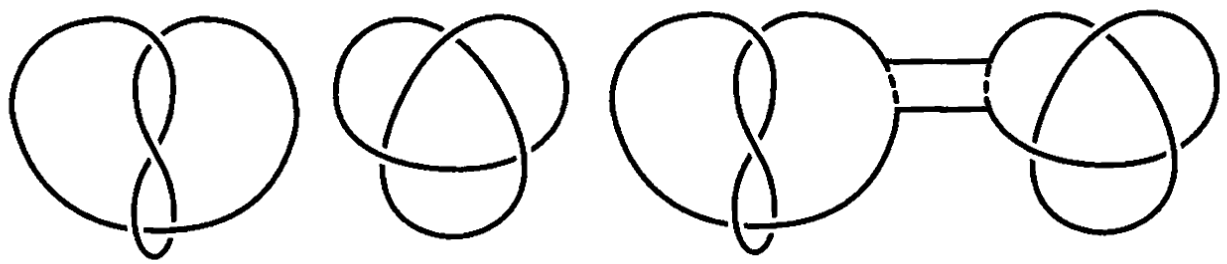
\includegraphics[width=0.8\linewidth]{ncomposicion}\\
	\caption[Composición de nudos]{Composición de nudos}
	\label{fig:composición}
\end{figure}

Para la formación de un nudo compuesto hay algunos consideraciones a tomar en cuenta: los nudos con los cuales se desea realizar la composición no deben estar superpuestos, los arcos que se eligen para remover no deben afectar los cruces del nudo original y los arcos introducidos para formar el nuevo nudo no deben formar nuevos cruces con el nudo original. 

\begin{figure}[ht]
	\centering
	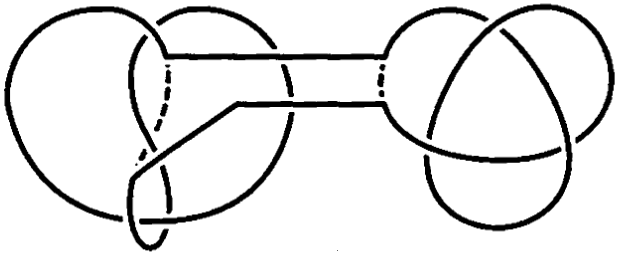
\includegraphics[width=0.4\linewidth]{nnocom}\\
	\caption[Ejemplo de como no se realiza la composición de nudos]{Ejemplo de como no se realiza la composición de nudos}
	\label{fig:nocom}
\end{figure}	

\begin{defn}\label{dfcp8} Un nudo es llamado \textbf{compuesto} si puede ser expresado como la composición de dos nudos, donde ninguno de los nudos por los cuales está formado son el nudo trivial y los nudos por los cuales está formado son llamados \textbf{nudos factor}. 
\end{defn}

El pedir que ninguno de los nudos factor sea el nudo trivial es porque el nudo trivial bajo la composición de nudos es el análogo al $0$ en los reales bajo la suma, es decir, si denotamos al nudo trivial como $K$ y tomamos un nudo cualesquiera $J$ tendríamos $J\# K=K\# J=J$. Entonces esto indicaría que cualquier nudo es un nudo compuesto.

\begin{figure}[ht]
	\centering
	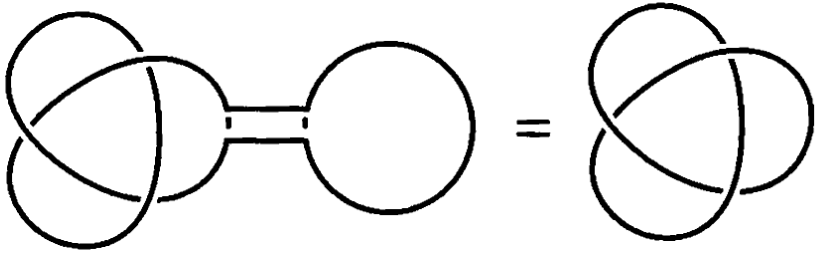
\includegraphics[width=0.6\linewidth]{ncomtriv}\\
	\caption[composición de un nudo con el nudo trivial]{Composición con el nudo trivial}
	\label{fig:comtriv}
\end{figure}

\begin{defn}\label{dfcp9} Un nudo que no es composición de cualesquiera dos nudos no triviales es llamado \textbf{nudo primo}.
\end{defn}

Para el trabajo con nudos compuestos es necesario resolver la siguiente pregunta ¿El nudo trivial es compuesto? En la figura \ref{fig:nudotrivial} podríamos pensar que no es un nudo compuesto, pero tal vez existe otra forma de proyectar el nudo trivial que contradiga esto.

\begin{prp}\label{prop1} El nudo trivial es un nudo primo.
\end{prp}

\begin{proof} Supongamos que el nudo trivial es un nudo compuesto, es decir, es la composición de por lo menos dos nudos distintos del nudo trivial. Sabemos que podemos pensar en cualquier nudo como la composición del nudo trivial con el mismo nudo, entonces como estamos suponiendo que el nudo trivial es compuesto tenemos que cualquier nudo puede ser visto como la composición de él mismo con los componentes del nudo trivial y esto implicaría que cualquier nudo es compuesto, lo cual es imposible.
\end{proof}

Este resultado es análogo a pensar en el $1$ en los naturales con el producto, es decir, la única forma de realizar la composición de dos nudos y esta nos regrese el nudo trivial es que los nudos con los que se realiza la composición son equivalentes al nudo trivial.

Pero a diferencia de los números naturales donde el orden de los factores no altera el producto, en la composición de nudos es posible poder formar distintos nudos compuestos del mismo par de nudos. Esto es posible al elegir distintos arcos que suprimir o darle otra orientación al nudo.

\begin{defn}\label{dfcp10} Una \textbf{orientación} es una elección para viajar a través del diagrama del nudo. Esta dirección es denotada en el diagrama por flechas. A un nudo provisto de una orientación le llamaremos \textbf{nudo orientado}.
\end{defn}

\begin{figure}[ht]
	\centering
	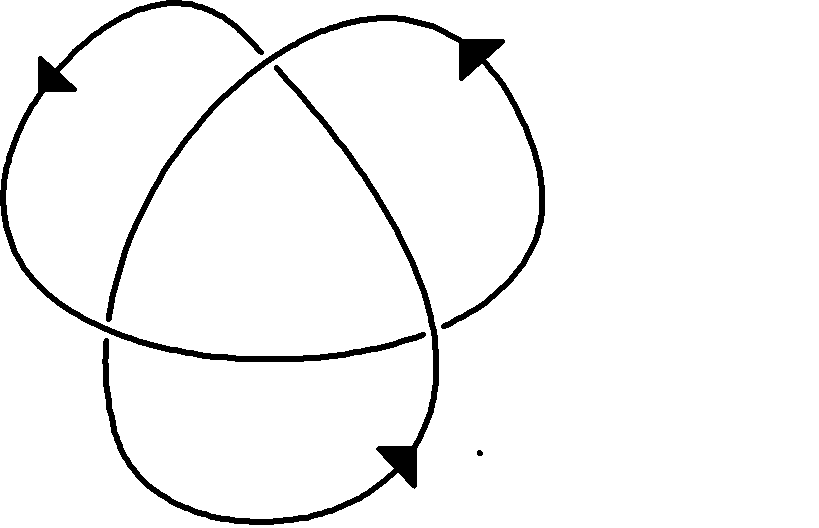
\includegraphics[width=0.3\linewidth]{orientado}\\
	\caption[Nudo trébol orientado]{Nudo trébol orientado}
	\label{fig:orientado}
\end{figure}

Entonces para cualesquiera par de nudos orientados $J$ y $K$, existen dos posibilidades de composición: La orientación sobre $J$ coincide con la orientación sobre $K$ en $J\#K$, resultando en una orientación para $J\#K$; o la orientación sobre $J$ y sobre $K$ no coinciden en $J\# K$. Todas las composiciones de dos nudos cuya orientación coincide producen el mismo nudo, análogamente para las composiciones cuya orientación no coincide.

\begin{figure}[ht]
	\centering
	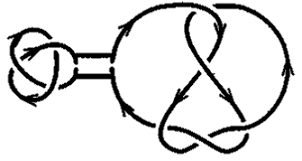
\includegraphics[width=0.3\linewidth]{ncoinciden}\\
	\caption[Composición de dos nudos cuyas orientaciones coinciden]{Composición de dos nudos cuyas orientaciones coinciden}
	\label{fig:coinciden}
\end{figure}

\begin{figure}[ht]
	\centering
	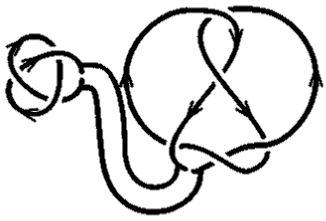
\includegraphics[width=0.35\linewidth]{nnocoinciden}\\
	\caption[Composición de dos nudos cuyas orientaciones no coinciden]{Composición de dos nudos cuyas orientaciones no coinciden}
	\label{fig:nocoinciden}
\end{figure}

Es posible que los nudos compuestos cuyas orientaciones coinciden sean los mismos que los nudos compuestos cuyas orientaciones no coinciden, para ello es necesario el concepto de nudo invertible.

\begin{defn}\label{dfcp11} Diremos que un nudo orientado es \textbf{invertible} si es equivalente a sí mismo pero con la orientación en sentido contrario.
\end{defn}

Si realizamos la composición de un nudo orientado invertible con un nudo orientado cualesquiera tendríamos que su composición cuando la orientación concuerda y cuando la orientación no concuerda es la misma.

\begin{defn}\label{dfcp28} El \textbf{anverso} de un nudo $K$ es la imagen de espejo de $K$ y es denotado por $\overline{K}$.
\end{defn}

Un nudo cualesquiera puede o no ser equivalente a su anverso.

\begin{defn}\label{dfcp29} Un nudo que es equivalente a su anverso es llamado \textbf{anfiquiral}\footnote{El termino anfiquiral es comúnmente usado por matemáticos, pero algunos químicos suelen usar el termino \textbf{aquiral} en referencia a lo mismo.}.
\end{defn}

Un ejemplo de un nudo que no es anfiquiral es el nudo trébol debido a que no es equivalente a su anverso, figura~\ref{fig:chiral}.

\begin{figure}[ht]
	\centering
	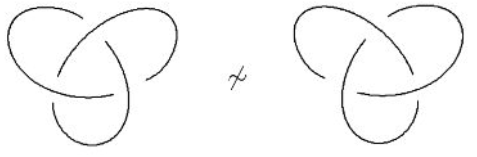
\includegraphics[width=0.5\linewidth]{chiral}\\
	\caption[Nudo no anfiquiral]{Nudo no anfiquiral}
	\label{fig:chiral}
\end{figure}

La prueba de que efectivamente este nudo no es anfiquiral la realizaremos más adelante.

\subsection{Enlaces}
Hasta el momento hemos restringido nuestra atención a los nudos, que puede ser visto como un lazo anudado, es decir, una cuerda entrelazada consigo misma y unida en sus extremos. Pero no hay razones para decir que se puede trabajar con un solo lazo.

\begin{defn}\label{dfcp12} Un \textbf{enlace} es una colección finita de nudos posiblemente enlazados entre sí. Análogo a lo conocido para nudos decimos que dos enlaces son el mismo o son \textbf{equivalentes} si podemos deformar uno en el otro de manera continua.
\end{defn}

Algunos ejemplos de enlaces simples conocidos son los llamados \textbf{enlaces de Whitehead}, figura~\ref{fig:whitehead}. Estos enlaces están formados por dos bucles anudados.

\begin{figure}[ht]
	\centering
	\includegraphics[width=0.5\linewidth]{nwhitehead}\\
	\caption[Enlaces de Whitehead]{Enlaces de Whitehead}
	\label{fig:whitehead}
\end{figure}

\begin{defn}\label{dfcp13} Llamaremos \textbf{componente} de un enlace a cada bucle anudado (nudo) del cual esta formado el enlace.
\end{defn}

Podríamos considerar un nudo como un enlace de un solo componente. Dado que los enlaces de Whitehead están hechos de dos bucles anudados diremos que es un enlace con dos componentes. Otro ejemplo de enlace simple son llamados \textbf{anillos de Borromeo}.

\begin{figure}[ht]
	\centering
	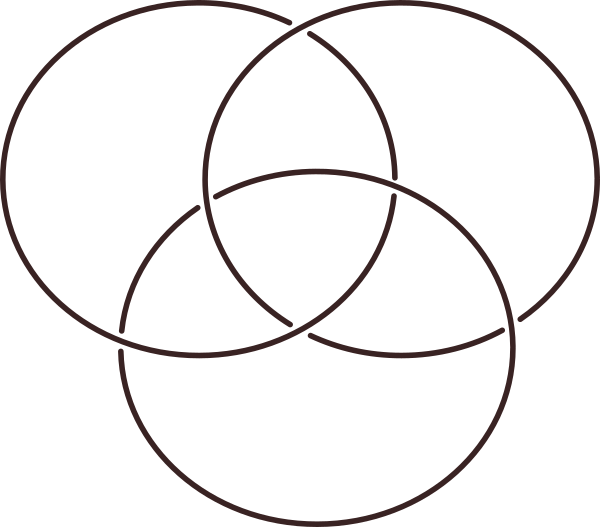
\includegraphics[width=0.2\linewidth]{borromean}\\
	\caption[Anillos de Borromeo]{Anillos de Borromeo}
	\label{fig:borromean}
\end{figure}

\begin{defn}\label{dfcp14} Un enlace es llamado \textbf{dividible} si los componentes del enlace pueden ser deformados de modo que se encuentren en diferentes lados del plano en el espacio tridimensional. 
\end{defn}

Existe una forma rápida de decir que dos enlaces no son el mismo, simplemente verificando el número de componentes que poseen. Pero no siempre trabajaremos con enlaces con diferente número de componentes, estamos interesados en saber cuando dos enlaces de igual número de componentes son distintos.

Un ejemplo inicial está dado por los enlaces más simples de dos componentes, el primero conocido como \textbf{enlace trivial} y el segundo \textbf{enlace de Hopf}, figura~\ref{fig:enlacetrivial}. Estos enlaces difieren el uno del otro debido a que el primero es dividible mientras que el segundo no.

\begin{figure}[ht]
	\centering
	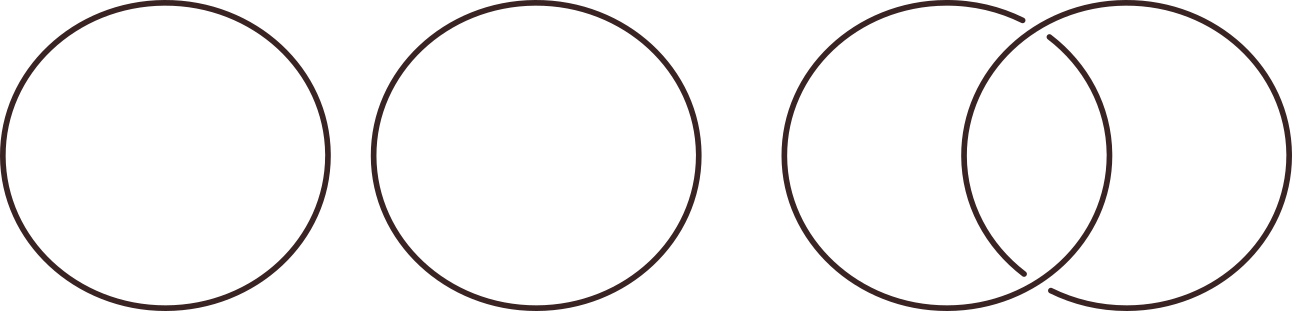
\includegraphics[width=0.55\linewidth]{enlacetrivial}\\
	\caption[Enlace trivial y enlace de Hopf]{Enlace trivial y enlace de Hopf}
	\label{fig:enlacetrivial}
\end{figure}

Sean $M$ y $N$ dos componentes en un enlace y elegimos una orientación en cada uno de ellos. Entonces a cada cruce entre las dos componentes se le puede asignar un $+1$ o un $-1$ dependiendo del caso (figura \ref{fig:numero}).

\begin{figure}[ht]
	\centering
	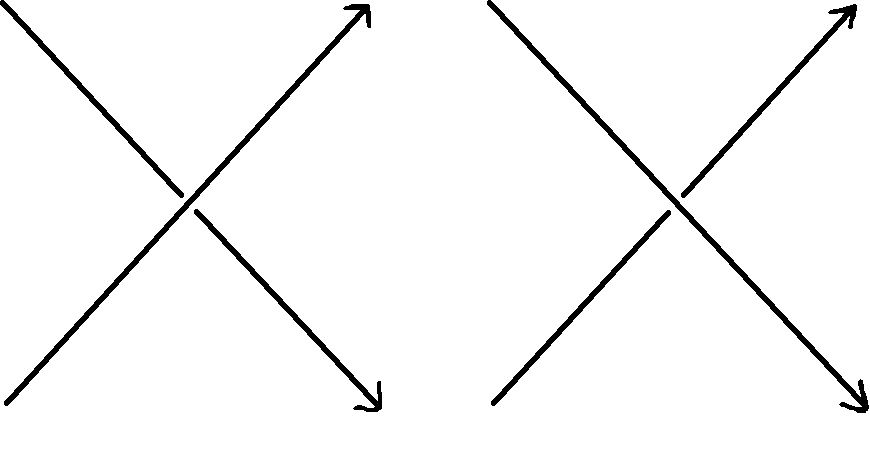
\includegraphics[width=0.35\linewidth]{numero}\\
	\caption[Enlaces]{Enlaces}
	\label{fig:numero}
\end{figure}

En la figura~\ref{fig:numero}, si tenemos un cruce del primer tipo (izquierda) se le asigna un $-1$ mientras que para el segundo tipo (derecha) se le asigna un $+1$.

\begin{defn}\label{dfcp15} Sea $L$ un enlace orientado y sea $M$ el conjunto de todos los cruces en $L$ con su respectivo valor, entonces el \textbf{número de enlace} de $L$ es la suma de todos los valores de los cruces en $M$ dividido entre 2.
\end{defn}

Por ejemplo el enlace trivial tiene número de enlace 0, el  enlace Hopf tiene número de enlace 1 o -1 dependiendo de la orientación. Otro ejemplo es el mostrado en la figura \ref{fig:linking}.

\begin{figure}[ht]
	\centering
	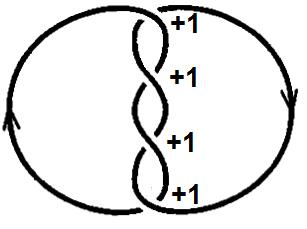
\includegraphics[width=0.2\linewidth]{nlinking}\\
	\caption[Número de enlace]{Número de enlace 2}
	\label{fig:linking}
\end{figure}

\begin{defn}\label{dfcp16} Un enlace es llamado \textbf{alternante} si en su diagrama las hebras van alternando entre arriba y abajo al recorrer el nudo en una dirección fija.
\end{defn}

Notemos que esta definición es análoga a la de nudo alternante, y así como esta algunas definiciones o teoremas son similares tanto en nudos como en enlaces.
\end{comment}
\begin{comment}
\section{Movimientos de Reidemeister}
Uno de los grandes problemas en la teoría de nudos es el clasificar los nudos, es decir, saber cuando un nudo es distinto a otro. En la sección anterior se habló brevemente de la equivalencia de nudos, pero trataremos de manera formal las definiciones antes dadas.

\begin{defn}\label{dfcp17} Sean $X$ y $Y$ espacios de Hausdorff. Una función $f:X\rightarrow Y$ es llamada una \textbf{incrustación} si $f:X\rightarrow f(X)$ es un homeomorfismo.
\end{defn}

\begin{defn}\label{dfcp18} Dos incrustaciones $f_0,f_1:X\rightarrow Y$ son \textbf{isotópicas} si existe una incrustación $F:X\times I \rightarrow Y\times I$ tal que $F(x,t)=(F(x,t),)$, $x\in X$, $t\in I=[0,1]$ con $f(x,0)=f_0(x)$, $f(x,1)=f_1(x)$. F es llamada \textbf{isotopía de conservación de nivel} o simplemente \textbf{isotopía}.
\end{defn}

Usaremos con frecuencia la notación $f_t(x)=f(x,t)$. Esta noción de isotopía no es buena en temas relacionados con los nudos, es por ello que necesitamos la siguiente definición:

\begin{defn}\label{dfcp19} Dos incrustaciones $f_0,f_1:X\rightarrow Y$ son \textbf{isotópicas en el espacio} si existe una isotopía $H:X\times I \rightarrow Y\times I$, $H(y,t)=(h_t(y),t)$, con $f_1=h_1f_0$ y $h_0=id_Y$. La función H es llamada un \textbf{isotopía espacial}.
\end{defn}

Una isotopía espacial define una isotopía $F$ que conecta $f_0$ con $f_1$ por $F(x,t)=(h_tf_0(x),t)$. La diferencia entre las dos definiciones anteriores es la siguiente: una isotopía transforma continuamente el conjunto $f_0(X)$ en $f_1(X)$ en Y, pero no toma en cuenta los puntos de $Y$ fuera de $f_1(X)$. Una isotopía espacial requiere que $Y$ se mueva continuamente junto con $f_t(X)$.

\begin{defn}\label{dfcp20} La \textbf{representación poligonal} de un nudo es la unión de los segmentos $[p_1,p_2],[p_2,p_3],...,[p_{n-1},p_n],[p_n,p_1]$ de un conjunto ordenado de distintos puntos $(p_1,p_2,...,p_n)$ formando el nudo.
\end{defn}

\begin{figure}[ht]
	\centering
	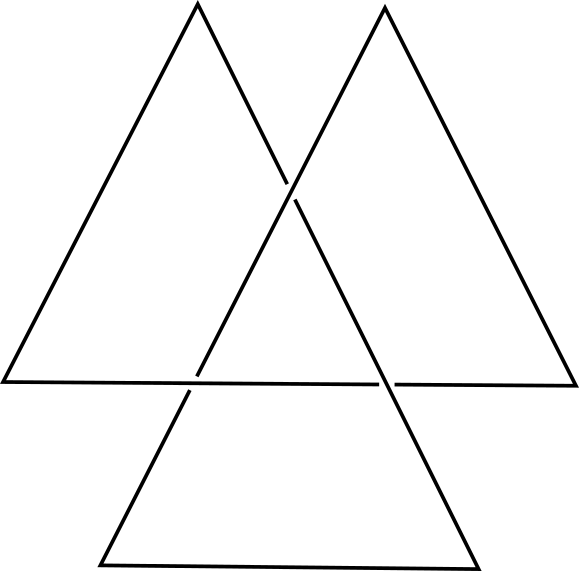
\includegraphics[width=0.3\linewidth]{poligonal}\\
	\caption[Representación poligonal del nudo trébol]{Representación poligonal del nudo trébol}
	\label{fig:poligonal}
\end{figure}

En ocasiones trabajaremos con la forma poligonal de un nudo, para ello utilizaremos la categoría p.l.\footnote{p.l. viene del inglés \textit{piecewise linear}} Los conceptos de isotopía e isotopía espacial son análogos a las definiciones anteriores para la categoría p.l.

\begin{defn}\label{dfcp22} Dos nudos (p.l.-nudos) son \textbf{equivalentes} si son isotópicos en el espacio (p.l.-isotópicos en el espacio).
\end{defn}

Los conceptos anteriores no son prácticos al trabajar, es por ello que trabajaremos dichos conceptos a través de movimientos en el espacio y en el plano.

\begin{defn}\label{dfcp23} Sea $u$ un segmento de un nudo poligonal $K$ en $\mathbb{R}^3$ y $D$ un triángulo en $\mathbb{R}^3$, $\partial D=u\cup v\cup w$, es decir, los lados de $D$ son $u$, $v$, $w$. Si $D\cap K=u$, entonces $K'=(K-u)\cup v\cup w$ define otro nudo poligonal. Diremos que $K'$ resulta de $K$ por un \textbf{$\Delta-$proceso} o un \textbf{$\Delta-$movimiento}. Si $K$ es orientado, $K'$ tiene que llevar la orientación inducida por $K$. El proceso inverso es denotado por $\Delta^{-1}$.
\end{defn}

\begin{figure}[ht]
	\centering
	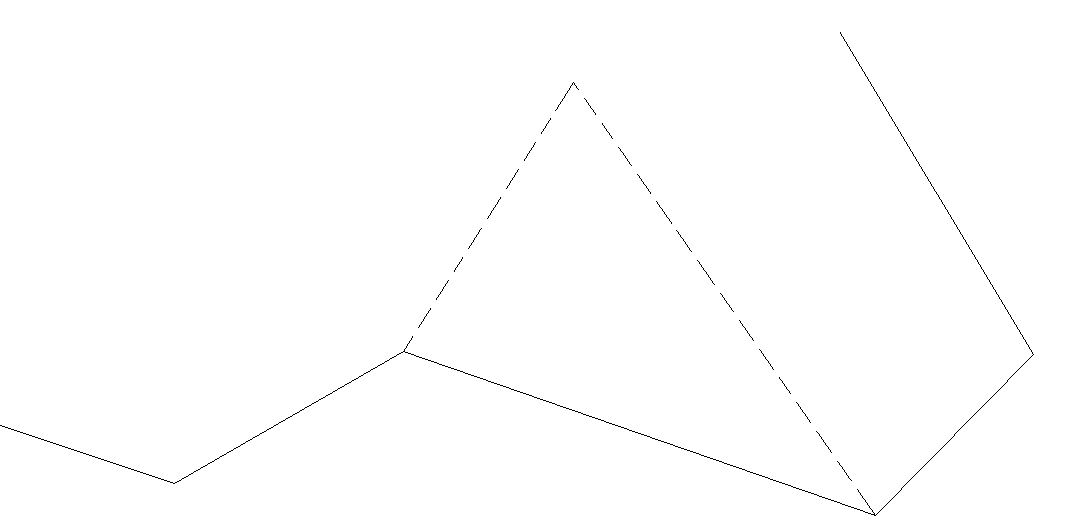
\includegraphics[width=0.6\linewidth]{tmov}\\
	\caption[$\Delta-$movimiento]{$\Delta-$movimiento}
	\label{fig:tmov}
\end{figure}

\begin{defn}\label{dfcp24} Dos nudos son \textbf{combinatóricamente equivalentes} o \textbf{isotópicos por movimientos}, si existe una sucesión finita de $\Delta-$movimientos o $\Delta^{-1}-$movimientos que transforma un nudo en el otro.
\end{defn}

Ya que tenemos distintas definiciones de equivalencia de nudos es necesario demostrar que estas definiciones son equivalentes. Para esto son necesarios algunos teoremas previos:

\begin{thm}\label{thm:schoenflies} (Alexander-Schoenflies) Sea $i:S^2\rightarrow S^3$ una incrustación (p.l.-incrustación). Entonces
	\begin{equation*}
		S^3=B_1\cup B_2,\text{ }  i(S^2)=B_1\cap B_2=\partial B_1=\partial B_2	
	\end{equation*}
donde $B_i$, $i=1,2$, es una 3-bola combinatórica ($B_i$ es p.l.-homeomorfa a un 3-tetraedro)
\end{thm}

%demostración pendiente, aún no la encuentro.

Este teorema corresponde al teorema de la curva de Jordan en dos dimensiones.

\begin{prp}\label{prp:Tietze} (Alexander-Tietze) Cualquier homeomorfismo (p.l.-homeomorfismo) $f$ de una n-bola $B$ que mantiene la frontera fija es isotópico a la identidad por una isotopía espacial (p.l.-isotopía espacial) que mantiene fija la frontera.
\end{prp}
%copia literal de la demostración, detalles pendientes
\begin{proof} 
	Definamos para $(x,t)\in \partial(B\times I)$ la siguiente función:
	\begin{equation*}
		H(x,t)=\left\{\begin{array}{lcc}
			x & si & t=0\\
			x & si & x\in\partial B\\
			f(x) & si & t=1
		\end{array}
		\right.
	\end{equation*}
	Cualquier punto $(x,t)\in B\times I$, $t>0$ está en un segmento recto en $B\times I$ uniendo un punto interior fijo $P$ de $B\times 0$ y un punto variable $X$ en $\partial(B\times I)$. Extendemos $H\mid\partial(B\times I)$ linealmente a lo largo de estos segmentos obteniendo un isotopía $H:B\times I\rightarrow B\times I$, en efecto, la isotopía espacial deseada. %colocar referencia
\end{proof}

\begin{figure}[ht]
	\centering
	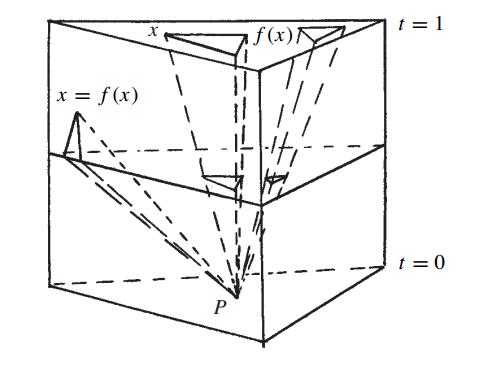
\includegraphics[width=0.3\linewidth]{tietze}\\
	\caption[Proposición de Alexander-Tietze]{Proposición de Alexander-Tietze}
	\label{fig:tietze}
\end{figure}

\begin{prp}\label{prp:equivalencia}
	Sean $K_0$, $K_1$ nudos (p.l.-nudos) en $S^3$ los siguientes enunciados son equivalentes:
	\begin{enumerate}
		\item Existe un homeomorfismo que preserva la orientación $f:S^3\rightarrow S^3$ que transforma $K_0$ en $K_1$, $f(K_0)=K_1$.
		\item $K_0$ y $K_1$ son equivalentes (isotópicos en el espacio).
		\item $K_0$ y $K_1$ son combinatóricamente equivalentes (isotópicos por movimientos).
	\end{enumerate}
\end{prp}

\begin{proof}
	$(1)\Rightarrow(2)$ Iniciaremos probando que existe una isotopía espacial $H(x,t)=(h_t(x),t)$ de $S^3$ tal que $h_1f$ deja fijo un 3-tetraedro $[P_0,P_1,P_2,P_3]$. Si $f:S^3\rightarrow S^3$ tiene un punto fijo, elijamos es te punto como $P_0$; sino, sea $P_0$ cualquier punto interior de un 3-tetraedro $[s^3]$ de $S^3$. Existe una isotopía espacial de $S^3$ que deja $\overline{S^3-[s^3]}$ fijo y lleva $P_0$ a cualquier otro punto interior de $[s^3]$. Si $[s^3]$ y $[s'^3]$ tienen una cara común, uno puede fácilmente construir una isotopía espacial que mueva un punto interior $P_0$ de $[s^3]$ a un punto interior $P_0'$ de $[s'^3]$ que es la identidad fuera de $[s^3]\cup[s'^3]$, figura~\ref{fig:equivalencia}.
	\begin{figure}[ht]
	\centering
	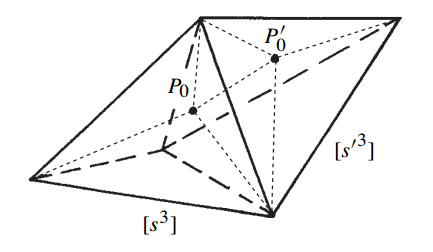
\includegraphics[width=0.4\linewidth]{equivalencia}\\
	\caption[Construcción de isotopía]{Construcción de isotopía}
	\label{fig:equivalencia}
	\end{figure}
	Así existe una isotopía espacial $H^0$ con $h_1^0f(P_0)=P_0$, desde que cualesquiera dos 3-tetraedros pueden ser conectados por una cadena de \textit{adjoining ones}. Luego elijamos un punto $P_1\neq P_0$ en el tetraedro de $P_0$, y por argumentos similares construimos una isotopía espacial $H_1$ con $h_1^1h_1^0f$ que deja fijo al 1-tetraedro $[P_0,P_1]$. Un paso más conduce a $h_1^2h_1^1h_1^0f$ con un 2-tetraedro $[P_0,P_1,P_2]$ fijo. En este momento la suposición viene en que f es necesario para preservar la orientación. Un punto $P_3\not\in [P_0,P_1,P_2]$, pero en la estrella de $[P_0,P_1,P_2]$, sería mapeado por $h_1^2h_1^1h_1^0f$ en un punto $P'^3$ en el mismo medio espacio con respecto al plano generado por $P_0$, $P_1$, $P_2$. Esto asegura la existencia de una isotopía espacial final $H^3$ tal que $h_1^3h_1^2h_1^1h_1^0f$ mantiene $[P_0,P_1,P_2,P_3]$ fijo. Esta afirmación se sigue del hecho que $H=H^3H^3H^1H^0$ es una isotopía espacial, $H(x,t)=(h_t(x),t)$. Por el teorema~\ref{thm:schoenflies} el complemento de $[P_0,P_1,P_2,P_3]$ es una 3-bola combinatórica y por la proposición~\ref{prp:Tietze} hay una isotopía espacial que conecta $h_1f$ con la identidad de $S^3$.
	
	$(2)\Rightarrow(1)$ consecuencia directa de la definición de isotopía espacial.
	
	$(1)\Rightarrow(3)$ Sean $K_0$ y $K_1$ nudos y sea $h:S^3\rightarrow S^3$ un homeomorfismo que preserva la orientación tal que $K_1=h(k_0)$. El argumento anterior muestra que hay otro homeomorfismo que preserva la orientación, $g:S^3\rightarrow S^3$ con $g(K_0)=K_0$, tal que $hg$ deja fijo algún 3-tetraedro $[s^3]$ que tendrá que ser elegido fuera de una vecindad regular de $K_0$ y $K_1$. Para un punto interior $P$ de $[s^3]$ consideremos $S^3-{P}$ como $\mathbb{R}^3$. Hay una traslación $\tau$ de $\mathbb{R}^3$, que mueve $K_0$ en $[s^3]-{P}$. Es fácil probar que $K_0$ y $\tau(K_0)$ son isotópicos por movimientos, figura~\ref{fig:equivalencia2}. Afirmamos que $K_1=hg(K_0)$ y $hg\tau(K_0)=\tau(K_0)$ son isotópicos por movimientos, que completaría la prueba: elijamos una subdivisión de la tiangulación de $S^3$ tal que los triángulos usados en la isotopía por movimientos entre $K_0$ y $\tau(K_0)$ forman un \textit{subcomplex} de $S^3$. Hay una isotopía por movimientos tal que $K_0\rightarrow\tau(K_0)$ que esta definida en los triángulos de la subdivisión. $hg:S^3\rightarrow S^3$ mapea el \textit{subcomplex} en otro que lleva la isotopía por movimientos.
	\begin{figure}[ht]
		\centering
		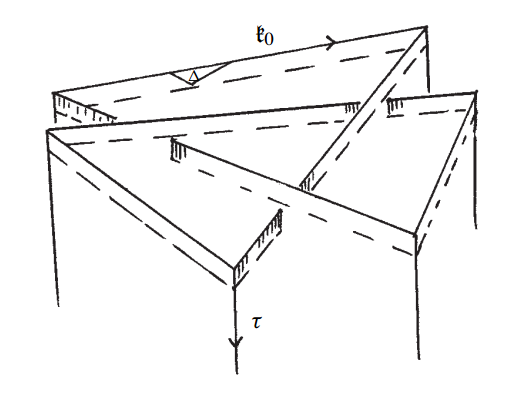
\includegraphics[width=0.4\linewidth]{equivalencia2}\\
		\caption[Isotopía por movimientos $K_0\rightarrow\tau(K_0)$]{Isotopía por movimientos $K_0\rightarrow\tau(K_0)$}
		\label{fig:equivalencia2}
	\end{figure}

	$(3)\Rightarrow(1)$ No es difícil de construir un homeomorfismo de $S^3$ en si mismo que realice un $\Delta^{\pm1}$-movimiento y deje fijo el resto del nudo. Elijamos una vecindad regular $U$ de un 2-tetraedro que define el $\Delta^{\pm1}$-movimiento cuya frontera coincide con el nudo en dos puntos. Por extensión lineal uno puede obtener un homeomorfismo que produzca el $\Delta^{\pm1}$-movimiento en $U$ y deje $S^3-U$ fijo.
\end{proof}

La descripción geometrica en el espacio tridimensional es realmente complicado. Por ello trabajaremos con los diagramas de nudos antes definidos, con la salvedad que lo antes definido como cruce en la definición~\ref{dfcp4} también es conocido como \textbf{punto múltiple}.

\begin{defn}\label{dfcp25} Una proyección $p$ de un nudo $K$ es llamada \textbf{regular} si
	\begin{enumerate}
		\item hay una cantidad finita de puntos múltiples (cruces) $\{P_i\mid1\le i\le n\}$, y todos los puntos múltiples son puntos dobles, es decir, $p^{-1}(P_i)$ contiene dos puntos de $K$,
		\item ningún vértice de $K$ es mapeado en un punto doble.
	\end{enumerate}
\end{defn}

\begin{figure}[ht]
	\centering
	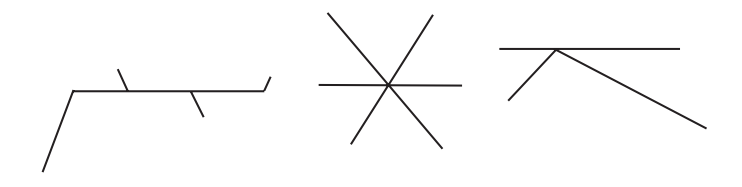
\includegraphics[width=0.8\linewidth]{noregular}\\
	\caption[Ejemplos de proyecciones no regulares]{Ejemplo de proyecciones no regulares}
	\label{fig:noregular}
\end{figure}

\begin{defn}\label{dfcp26} El mínimo número de puntos dobles o cruces en una proyección regular de un nudo es llamado el \textbf{orden} del nudo.
\end{defn}

El objetivo de trabajar con la proyección de un nudo es facilitar el trabajo, pero para ello debemos definir cuando dos diagramas son equivalentes.

\begin{defn}\label{dfcp27} Dos diagramas de nudo son llamados \textbf{equivalentes}, si están conectados por una sucesión finita de \textbf{movimientos de Reidemeister} $\Omega_i$, $i=1,2,3$, o sus inversos $\Omega_i^{-1}$
\end{defn}

\begin{figure}[ht]
	\centering
	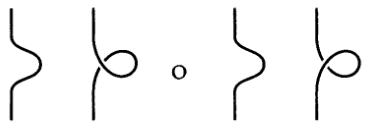
\includegraphics[width=0.5\linewidth]{R1}\\
	\caption[Movimiento de Reidemeister tipo 1 ($\Omega_1$)]{Movimiento de Reidemeister tipo 1 ($\Omega_1$)}
	\label{fig:R1}
\end{figure}

\begin{figure}[ht]
	\centering
	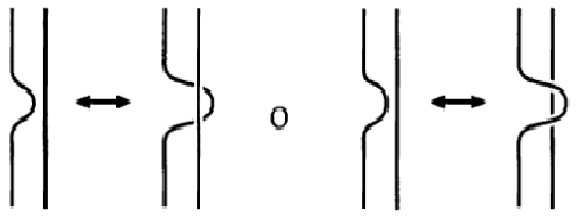
\includegraphics[width=0.5\linewidth]{R2}\\
	\caption[Movimiento de Reidemeister tipo 2 ($\Omega_2$)]{Movimiento de Reidemeister tipo 2 ($\Omega_2$)}
	\label{fig:R2}
\end{figure}

\begin{figure}[ht]
	\centering
	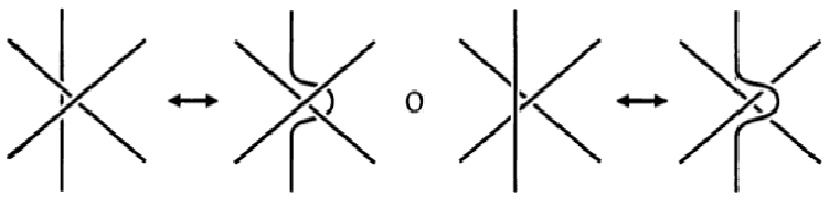
\includegraphics[width=0.6\linewidth]{R3}\\
	\caption[Movimiento de Reidemeister tipo 3 ($\Omega_3$)]{Movimiento de Reidemeister tipo 3 ($\Omega_3$)}
	\label{fig:R3}
\end{figure}

Notemos que las operaciones $\Omega_i^{\pm1}$ efectúan cambios locales en el diagrama, pero falta probar que estas operaciones pueden ser representadas por isotopías espaciales del nudo y viceversa.

\begin{prp}\label{prp:eq} Dos nudos son equivalentes si y sólo si sus diagramas son equivalentes.
\end{prp}

\begin{proof}
	El primer paso en la demostración sería verificar que cualesquiera dos proyecciones regulares $p_1$, $p_2$ del mismo nudo poligonal $K$ están conectados por $\Omega_i^{\pm1}$-movimientos. Sean $p_1$, $p_2$ representados por puntos en $S^2$, y elijamos en $S^2$ una trayectoria poligonal $s$ de $p_1$ a $p_2$ en posición general con respecto a las lineas de proyecciones singulares en $S^2$. Cuando se cruza dicha linea el diagrama será cambiado por una operación $\Omega_i^{\pm1}$, el tipo actual depende del tipo de la singularidad, correspondiente a la linea que se cruza.
	
	Queda mostrar que para una proyección fija nudos equivalentes poseen diagramas equivalentes. De acuerdo a la proposición~\ref{prp:equivalencia} es suficiente probar que un $\Delta^{\pm1}$-movimiento induce una $\Omega_i^{\pm1}$-operación en la proyección. Esto es verificado en la figura~\ref{fig:eq}.
	\begin{figure}[ht]
		\centering
		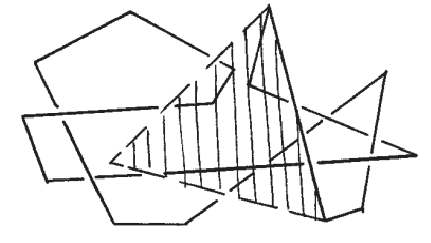
\includegraphics[width=0.5\linewidth]{eq}\\
		\caption[Equivalencia de diagramas]{Equivalencia de diagramas}
		\label{fig:eq}
	\end{figure}  
\end{proof}

Mostraremos un ejemplo de la utilización de los movimientos de Reidemeister.

\begin{figure}[ht]
	\centering
	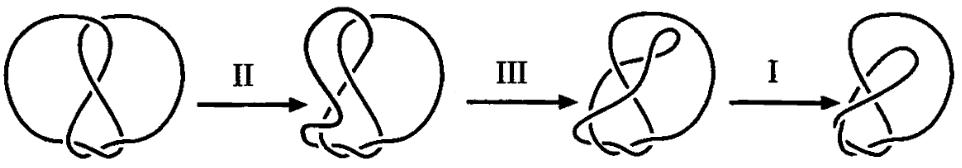
\includegraphics[width=0.7\linewidth]{mrp}\\
	\caption[Utilización de los movimientos de Reidemeister]{Utilización de los movimientos de Reidemeister}
	\label{fig:mrp}
\end{figure}

Notemos que aunque los movimientos de Reidemeister nos ayudan a demostrar cuando dos nudos son equivalentes, el método en general nos ayudara a probar cuando lo son pero no cuando no lo son, esto se debe a que para poder demostrar que dos nudos no son equivalentes a través de movimientos de Reidemeister es necesario probar toda posible combinación de movimientos en el nudos que tiende a ser un trabajo interminable.
\end{comment}
\begin{comment}
\section{Notación de Dowker y notación de Conway}
\subsection{Notación de Dowker}
La notación de Dowker es una forma simple de poder describir un diagrama de nudo. Iniciaremos dando dicha notación para un nudo alternante. Supongamos que tenemos un diagrama de un nudo que queremos describir entonces realizamos el siguiente procedimiento:
\begin{enumerate}
	\item Elegimos una orientación para el nudo.
	\item Nos posicionamos en cualquier cruce y lo etiquetamos con un 1.
	\item En el cruce que nos encontramos tomamos la hebra que pasa por debajo y empezamos a recorrer el nudo.
	\item Al encontrar un nuevo cruce lo etiquetamos con 2.
	\item Siguiendo el mismo camino por el que íbamos, etiquetamos el siguiente cruce con 3.
	\item Repetir el procedimiento y parar hasta que cada cruce posea dos etiquetas.
\end{enumerate}

\begin{figure}[ht]
	\centering
	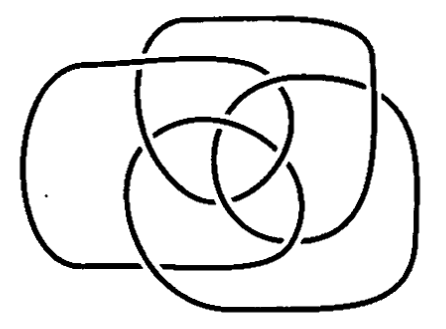
\includegraphics[width=0.275\linewidth]{alter}\\
	\caption{Un nudo Alternante}
	\label{fig:alter}
\end{figure}

\begin{figure}[ht]
	\centering
	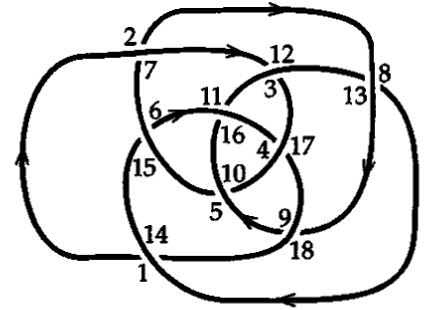
\includegraphics[width=0.275\linewidth]{etiqueta}\\
	\caption[Etiquetado de un nudo]{Etiquetado de la figura~\ref{fig:alter}}
	\label{fig:etiqueta}
\end{figure}

Notemos que el etiquetado le asigna a cada cruce un número par y uno impar, figura~\ref{fig:etiqueta}. Así podemos pensar en este etiquetado como una asignación de parejas de números entre $1$ y $2n$ con $n$ el numero de cruces. Para el caso de nuestro ejemplo obtenemos la tabla~\ref{tab:equiv}.

\begin{table}
	\centering
		\begin{tabular}{|c|c|c|c|c|c|c|c|c|}
			1 & 3 & 5 & 7 & 9 & 11 & 13 & 15 & 17 \\  
			14 & 12 & 10 & 2 & 18 & 16 & 8 & 6 & 4 \\ 
		\end{tabular}
	\caption{Correspondencia de números}
	\label{tab:equiv}
\end{table}

Notemos que los números impares están ordenados de forma ascendente mientras que los pares están desordenados, así pues podríamos simplificar esto y simplemente escribir $(14,12,10,2,18,16,8,6,4)$ y de esta forma guardar la información completa debido a que por el orden de los impares sabemos que $1$ esta emparejado con el $14$, el $3$ con el $12$ y así sucesivamente.

Así para un diagrama de nudo podemos obtener una sucesión de enteros pares, donde la cantidad de enteros pares debe coincidir con el numero de cruces del nudo.

\begin{defn}\label{dfcp30} Diremos que un conjunto formado por pares de números es \textbf{dibujable} si para cualesquiera dos ciclos definidos por un intervalo dado deben compartir uno o más segmentos, o intersectarse en un numero par de puntos sin incluir puntos iniciales y finales.
\end{defn}

\begin{prp}\label{prop:etiq} Siguiendo el procedimiento anterior para encontrar la notación de Dowker, a cada cruce le corresponde un número par y uno impar.
\end{prp}

\begin{proof}
	Consideremos un nudo dibujable en el cual existen $i$, $j$ etiquetas de un cruce de dicho nudo tales que tanto $i$ como $j$ son impares o pares, entonces tendríamos dos ciclos, digamos $i,i+1,...,j-1,j$ y $j,j+1,...,2n-1,2n,1,...,i$ que no comparten ningún segmento simplemente se cruzan en un número par de puntos incluidos los puntos iniciales y finales. Entonces tendríamos un conjunto de pares de números no dibujable, contradiciendo nuestra hipótesis.
\end{proof}

La proposición anterior es importante ya que sin ella la notación de Dowker no tendría sentido.

Sabemos como dado un diagrama de nudo encontrar su notación de Dowker, ahora supongamos que queremos obtener el diagrama del nudo dada la notación de Dowker. Para ello lo ejemplificaremos con el nudo $(8,10,12,2,14,14,6,4)$.

Iniciamos dibujando el primer cruce y etiquetándolo con 1 y 8. Extendemos la hebra que pasa por debajo del nudo y dibujamos el siguiente cruce, al cual le corresponde la etiqueta 2 y 7. Debido a que el nudo es alternante sabemos que la hebra que le corresponde al dos es una hebra que pasa por arriba. Seguimos este procedimiento hasta llegar a un número cuya etiqueta ya esta colocada, cuando llegamos a dicho número conectamos el el cruce en el cual nos encontramos con el que sigue (el número que ya estaba etiquetado).

\begin{figure}[ht]
	\centering
	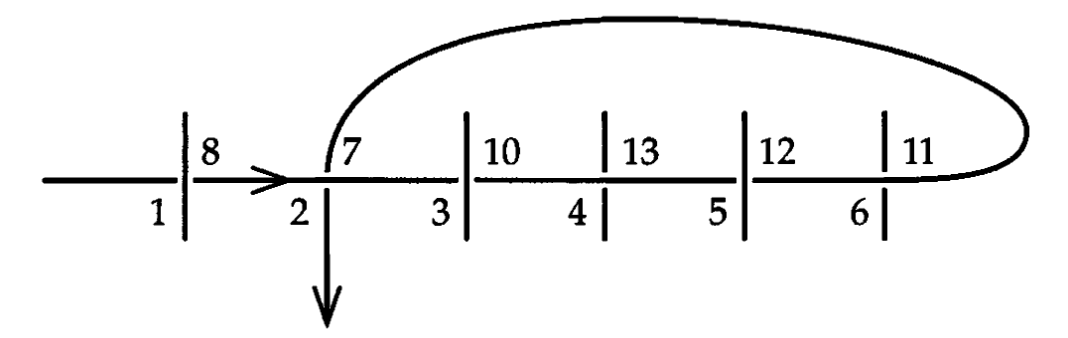
\includegraphics[width=0.5\linewidth]{dn1}
	\caption{De notación de Dowker a nudo}
	\label{fig:dn1}
\end{figure}

Continuamos con este procedimiento. Si encontramos una etiqueta no colocada con anterioridad simplemente tendríamos que agregar un nuevo cruce y etiquetarlo como corresponde, obteniendo el nudo como se quiere.

\begin{figure}[ht]
	\centering
	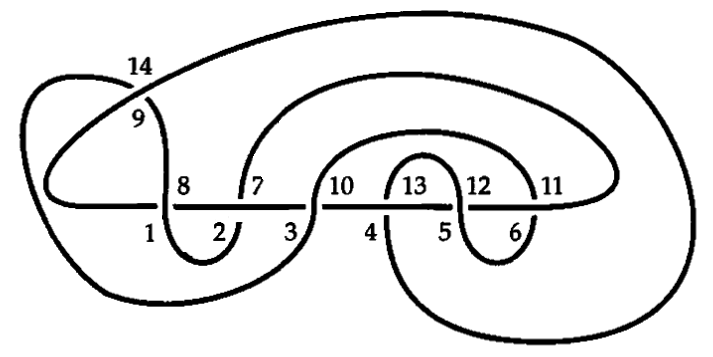
\includegraphics[width=0.4\linewidth]{dn2}
	\caption[De notación de Dowker a nudo]{De notación de Dowker a nudo, finalizado}
	\label{fig:dn2}
\end{figure}

Notemos que el procedimiento antes descrito es ambiguo, debido a las elecciones que se deben tomar de como formar los arcos en el nudo. Nuestras elecciones nos pueden llevar a nudos distintos, por ejemplo la sucesión $(4,6,2,10,12,8)$ puede representar dos nudos distintos como sigue:

\begin{figure}[ht]
	\centering
	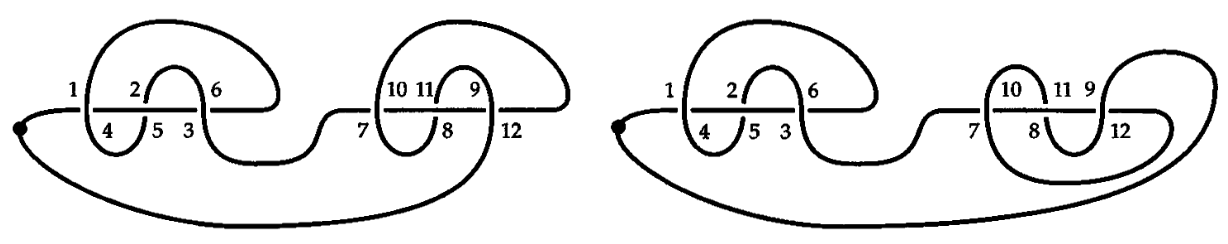
\includegraphics[width=0.8\linewidth]{dn3}
	\caption[Ambigüedad en la notación de Dowker]{Ambigüedad en la notación de Dowker}
	\label{fig:dn3}
\end{figure}

Notemos que estos dos nudos son nudos compuestos, y esto se ve reflejado en el hecho que la sucesión $(4,6,2,10,16,8)$ es realmente un corrimiento de los números $4$, $6$, $2$. Es decir, cuando la permutación de los números pares puede ser descompuesta en dos subpermutaciones separadas el resultado es un nudo compuesto (asumiendo que cada factor sea un nudo no trivial). Sin embargo, si nos limitamos a sucesiones de números pares que no puedan ser divididos en subpermutaciones, el resultado será un nudo particular o su imagen de espejo.

\begin{figure}[ht]
	\centering
	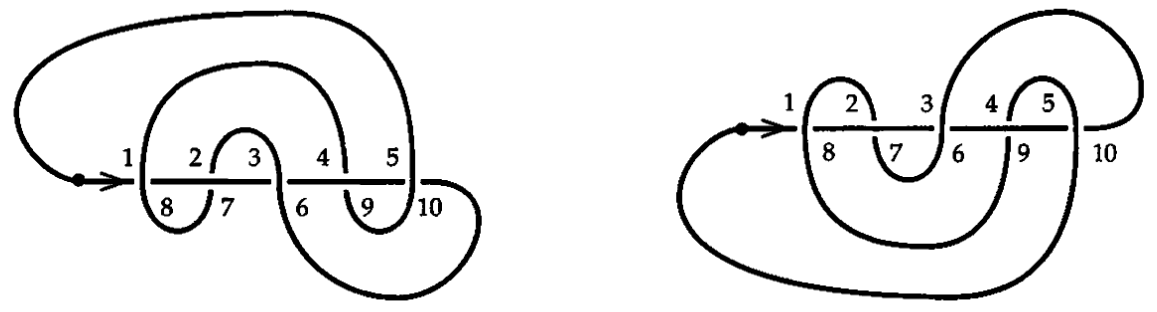
\includegraphics[width=0.7\linewidth]{dn4}
	\caption[Un nudo y su imagen de espejo]{Un nudo y su imagen de espejo ambos dados por $(8,6,10,2,4)$}
	\label{fig:dn4}
\end{figure}

En particular para un nudo anfiquiral la notación de Dowker nos produce un único nudo.

Recordemos que el procedimiento explicado con anterioridad esta hecho para nudos alternantes, pero este mismo procedimiento puede ser extendido a nudos que no son alternantes. Añadimos signos $+$ y $-$ en nuestra sucesión de números pares y modificando las reglas como sigue: El etiquetado se hace exactamente de la misma manera, pero si el entero par es asignado a un cruce que pasa por arriba colocaremos el signo $+$ precediendo a la etiqueta, mientas que si el número par es asignado a un cruce que pasa por abajo colocaremos el signo $-$ precediendo a la etiqueta.

\begin{figure}[ht]
	\centering
	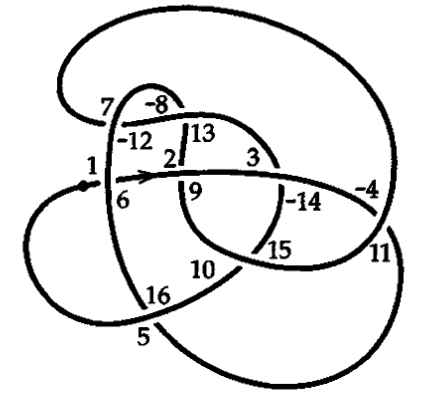
\includegraphics[width=0.25\linewidth]{dn5}
	\caption[Notación de Dowker, nudo no alternante]{Notación de Dowker, nudo no alternante}
	\label{fig:dn5}
\end{figure}

Entonces tendríamos que la notación de Dowker para el nudo de la figura~\ref{fig:dn5} es $(+6,-14,+16,-12,+2,-4,-8,10)$.

La notación de Dowker nos permite obtener diagramas de nudos al tener una simple sucesión de números pares. En particular, supongamos que queremos intentar clasificar los nudos de 14 cruces, el número de sucesiones de 14 números $2$, $4$, $6$, $8$, $10$, $12$, $14$, $16$, $18$, $20$, $22$, $24$, $26$, $28$ es $14!$, que es alrededor de $87$ billones. Además podemos colocar $+$ o $-$ antes de cada número obteniendo así otro factor de $2^{14}$.

\subsection{Notación de Conway} 
Esta notación es importante debido a que ha sido utilizada para probar numerosos resultados y además, recientemente, ha sido aplicada en los resultados en ADN concernientes a la teoría de nudos. Esta notación es particularmente útil en los cálculos que involucran lo que llamaremos \textbf{enredo}.

\begin{defn}\label{dfcp31} Un \textbf{enredo} en el diagrama de un nudo o enlace es una región en el diagrama que se puede rodear por un círculo tal que el nudo o enlace cruza al círculo exactamente 4 veces, los cuatro puntos de intersección son conocidos como los \textbf{puntos finales} del enredo. 
\end{defn}

\begin{figure}[ht]
	\centering
	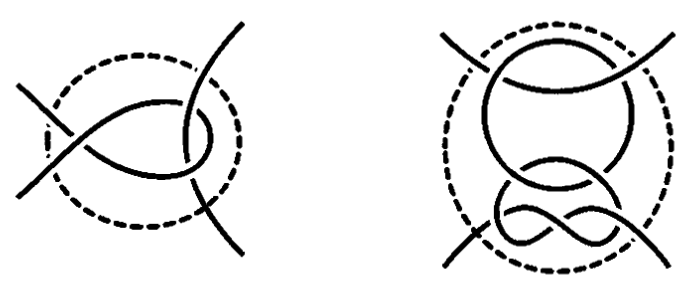
\includegraphics[width=0.4\linewidth]{cn1}
	\caption[Enredos]{Enredos}
	\label{fig:cn1}
\end{figure}

Pensaremos en los cuatro puntos donde el nudo o enlace cruza al circulo como las cuatro direcciones de una brújula $NO$, $NE$, $SO$, $SE$. En un nudo o enlace los enredos no necesariamente son únicos, es decir, en un mismo nudo o enlace podemos construir distintos bloques de enredos, figura~\ref{fig:cn2}.

\begin{figure}[ht]
	\centering
	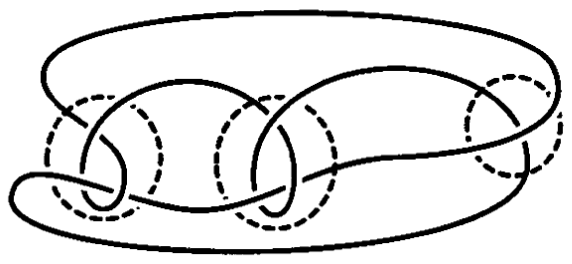
\includegraphics[width=0.4\linewidth]{cn2}
	\caption[Enredos en un nudo o enlace]{Enredos en un nudo o enlace}
	\label{fig:cn2}
\end{figure}

\begin{defn}\label{dfcp32} Diremos que dos enredos son equivalentes si podemos transformar uno en el otro de forma continua mientras los cuatro puntos que intersectan al círculo permanecen fijos y ademas al realizar los movimientos el enredo no sale del círculo.
\end{defn}

\begin{figure}[ht]
	\centering
	
\includegraphics[width=0.9\linewidth]{cn3}
	\caption[Enredos equivalentes]{Enredos equivalentes}
	\label{fig:cn3}
\end{figure}

Notemos que dado un enredo podemos formar un nudo simplemente uniendo a pares los puntos finales, por ejemplo tomando el primer enredo de la figura anterior podemos obtener:

\begin{figure}[ht]
	\centering
	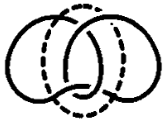
\includegraphics[width=0.175\linewidth]{cn4}
	\caption{Nudo obtenido del enredo en la figura~\ref{fig:cn3}}
	\label{fig:cn4}
\end{figure}

Entonces podemos decir que dos nudos son equivalentes cuando enredos correspondientes sean equivalentes. Uno de los enredos mas simples esta formado simplemente por dos cadenas verticales, figura~\ref{fig:cn5}a, conocido como el \textbf{enredo $\infty$}. Análogamente tenemos un enredo formado por dos cadenas horizontales, figura~\ref{fig:cn5}b, conocido como el \textbf{enredo $0$}.

\begin{figure}[ht]
	\centering
	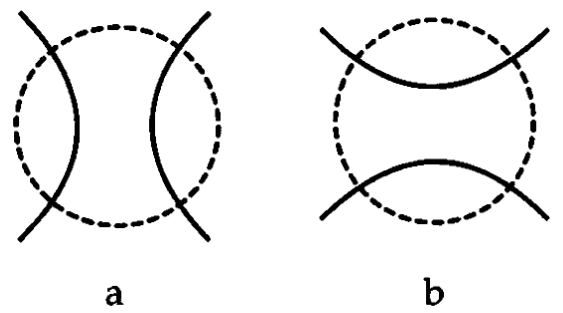
\includegraphics[width=0.35\linewidth]{cn5}
	\caption[Enredo $\infty$ y enredo $0$]{Enredo $\infty$ y enredo $0$}
	\label{fig:cn5}
\end{figure}

También podemos formar enredos de la siguiente manera: consideremos dos trozos de cuerda colocados de manera horizontal uno frente a otro, si enrollamos una cantidad $n$ de veces las cuerdas entre ellas mismas formamos un enredo llamado el \textbf{enredo $n$}, por ejemplo para el caso de $n=3$ obtenemos la figura~\ref{fig:cn6}.

\begin{figure}[ht]
	\centering
	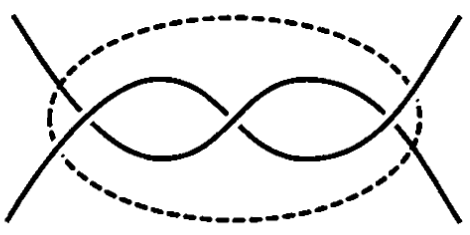
\includegraphics[width=0.35\linewidth]{cn6}
	\caption[Enredo $3$]{Enredo $3$}
	\label{fig:cn6}
\end{figure}

Construiremos enredos más complicados a partir del enredo $3$. Primero podemos formar un enredo tal que sea la reflexión del enredo $3$ respecto a la diagonal formada a partir de los puntos $NO$ y $SE$. Notemos que los dos puntos finales del enredo que pertenecen a la diagonal se mantienen fijos cuando realizamos la reflexión, mientras que los puntos finales en el enredo que no pertenecen a la diagonal son intercambiados.

\begin{figure}[ht]
	\centering
	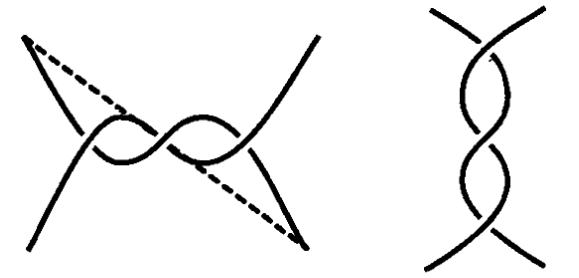
\includegraphics[width=0.35\linewidth]{cn7}
	\caption[Reflexión del enredo $3$]{Reflexión del enredo $3$}
	\label{fig:cn7}
\end{figure}

También podemos considerar la unión o concatenación de dos enredos, por ejemplo tomemos el nudo antes formado y juntemos sus puntos finales con los puntos finales del enredo $2$, así formamos el enredo $3$ $2$, figura~\ref{fig:cn8}.

\begin{figure}[ht]
	\centering
	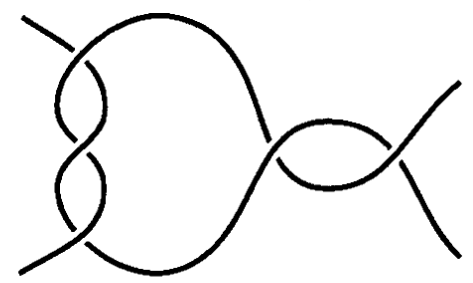
\includegraphics[width=0.3\linewidth]{cn8}
	\caption[Enredo $3$ $2$]{Enredo $3$ $2$}
	\label{fig:cn8}
\end{figure}

De esta forma podemos formar distintos tipos de enredos, algunos ejemplos se presentan en la figura~\ref{fig:cn9}.

\begin{figure}[ht]
	\centering
	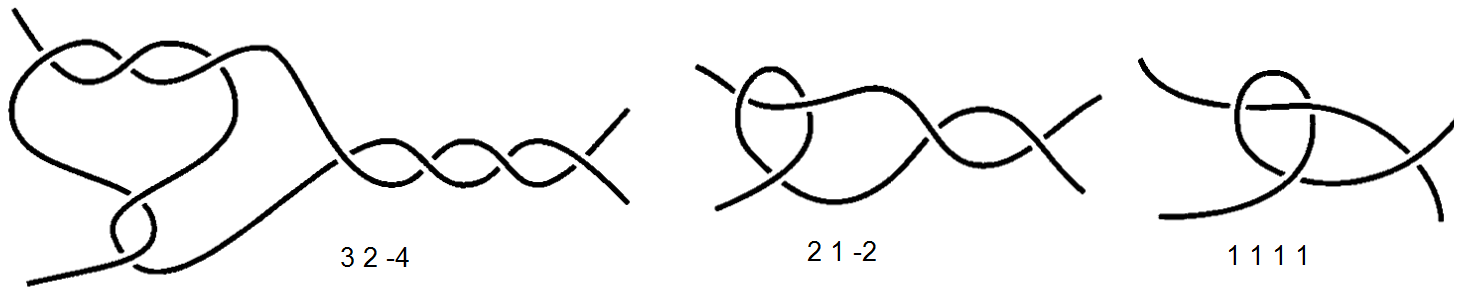
\includegraphics[width=0.9\linewidth]{cn9}
	\caption{Distintos ejemplos de enredos}
	\label{fig:cn9}
\end{figure}

\begin{defn}\label{dfcp33} A cualquier enredo que puede ser construido con el procedimiento anterior es llamado un \textbf{enredo racional}.
\end{defn}

Notemos que si un enredo racional es representado por un número par de enteros, podemos pensar en construirlo simplemente iniciando con dos cuerdas verticales (el enredo $\infty$) y luego girar los dos puntos finales inferiores uno alrededor del otro un cierto número de veces, mientras los puntos finales superiores permanecen fijos. También podríamos enrollar los dos puntos finales derechos mientras los izquierdos se mantienen fijos.

Similarmente, si el enredo racional es representado por un numero impar de enteros, podemos construirlo iniciando con dos cuerdas horizontales (el enredo $0$) y realizar un procedimiento similar al del caso par.

Consideremos un enredo racional dado por $a_1a_2...a_n$, donde $a_i$ es un entero para cualquier subíndice $i$, existe una forma de representar dicho enredo de una forma más simple, el procedimiento es el siguiente:
\begin{enumerate}
	\item Tomemos el primer entero $a_1$ y consideremos la fracción $\frac{1}{a_1}$.
	\item A la fracción obtenida en el paso anterior le sumamos el siguiente entero de la sucesión, $a_2$, obteniendo $a_2+\frac{1}{a_1}$.
	\item Lo obtenido en el paso anterior lo consideramos el denominador de una nueva fracción cuyo numerador es $1$ obteniendo $\frac{1}{a_2+\frac{1}{a_1}}$.
	\item Repetir los pasos 2 y 3 hasta no tener números en la sucesión.
\end{enumerate}

Por ejemplo, consideremos el enredo $-2$ $3$ $2$ entonces obtenemos $2+\frac{1}{3+\frac{1}{-2}}$.

\begin{defn}\label{dfcp34} La fracción obtenida del procedimiento anterior es conocida como la \textbf{fracción continua} asociada a un enredo.
\end{defn}

Notemos que al operar la fracción continua de un enredo, este se transforma en un sólo número racional. Es decir, a cada enredo se le puede asignar un número racional que lo represente. Tomemos el enredo usado como ejemplo anteriormente, tenemos lo siguiente:

\[
2+\frac{1}{3+\frac{1}{-2}}=2+\frac{2}{5}=\frac{12}{5}
\]

Así pues tenemos que $\frac{12}{5}$ es el racional asociado al enredo $-2$ $3$ $2$.

\begin{prp}\label{prop:eeq} Dos enredos racionales son equivalentes si y sólo si sus respectivos números racionales asociados son el mismo.
\end{prp}

\begin{defn}\label{dfcp35} Un \textbf{enlace racional} es el enlace resultante al cerrar los puntos finales de un enredo racional.
\end{defn}

Por ejemplo el nudo ocho es un nudo racional, el enredo que genera a dicho nudo es el enredo $2$ $2$. Podemos usar la notación para enredos racionales para denotar al correspondiente nudo o enlace racional. Llamaremos a esta notación la \textbf{notación de Conway}.

Podemos usar los enredos racionales para construir enredos más complicados, para ello definiremos una forma de "multiplicar" dos enredos para obtener uno nuevo.

\begin{defn}\label{dfcp36} Sean $K_1$ y $K_2$ dos enredos, consideremos la reflexión del enredo $K_1$ con respecto a la diagonal que pasa por los puntos $NO$ y $SE$. Entonces unimos los extremos del enredo resultante con $K_2$ y obtenemos un nuevo enredo llamado \textbf{multiplicación} de $K_1$ y $K_2$
\end{defn}

\begin{figure}[ht]
	\centering
	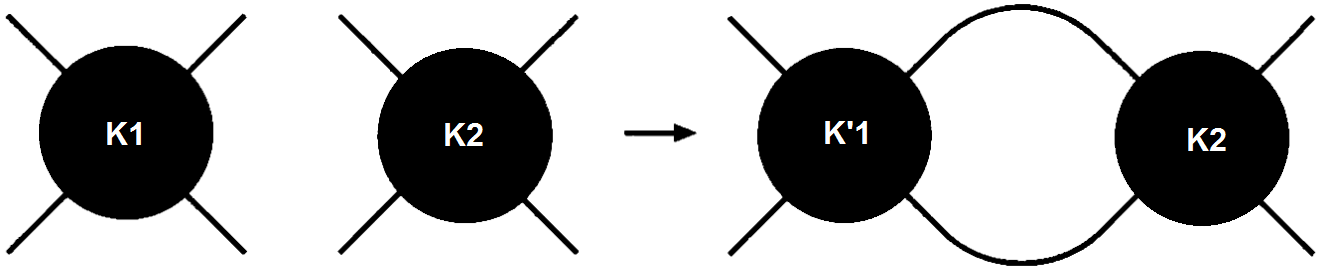
\includegraphics[width=0.65\linewidth]{cn10}
	\caption[Multiplicación de enredos]{Multiplicación de enredos}
	\label{fig:cn10}
\end{figure}

Podemos pensar que el enredo racional $3$ $2$ se forma multiplicando los enredos $3$ y $2$. Notemos que la multiplicación de enredos racionales nos da un enredo racional, es más si realizamos la multiplicación de cualquier enredo con el enredo $0$ el resultado es la reflexión del enredo original respecto a la diagonar que pasa por los puntos $NO$ y $SE$.

\begin{defn}\label{defcp37} Sean $K_1$ y $K_2$ dos enredos, la \textbf{suma} de estos enredos es la concatenación o unión de los enredos.
\end{defn}

\begin{figure}[ht]
	\centering
	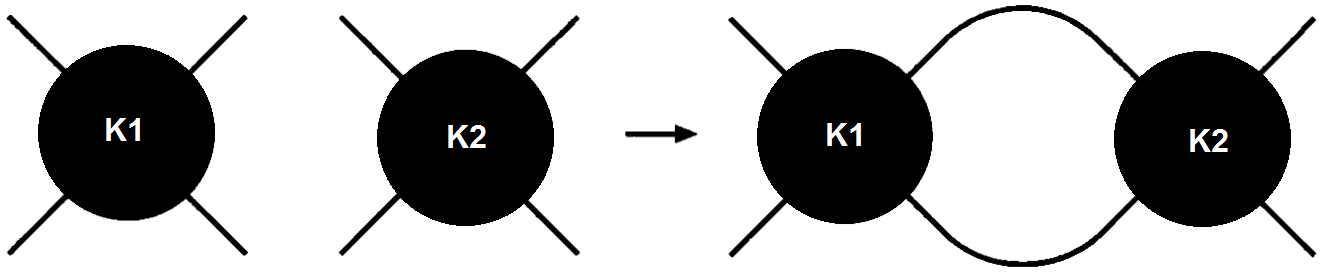
\includegraphics[width=0.7\linewidth]{cn11}
	\caption[Suma de enredos]{Suma de enredos}
	\label{fig:cn11}
\end{figure}

Si multiplicamos cada enredo de una sucesión de enredos por el enredo $0$ y los sumamos entre sí, denotamos el enredo resultante por la sucesión de números que correspondían a los enredos originales, pero ahora separados por comas. Por ejemplo, en la figura~\ref{fig:cn12} se muestra el nudo $8_5$, este enredo es escrito como $30+30+20$ o simplemente $3,3,2$.

\begin{figure}[ht]
	\centering
	
\includegraphics[width=0.175\linewidth]{ncn12}
	\caption[Nudo $8_5$]{Nudo $8_5$}
	\label{fig:cn12}
\end{figure}

\begin{defn}\label{dfcp37} Un nudo obtenido de un enredo representado por un número finito de enteros separados por comas es llamado nudo \textbf{pretzel}.
\end{defn}

\begin{defn}\label{dfcp38} Diremos que un enredo es \textbf{algebraico} si puede ser obtenido mediante operaciones de suma y multiplicación de enredos racionales. Análogamente un enlace es llamado \textbf{algebraico}\footnote{En ocasiones un enlace algebraico también es llamado un \textbf{enlace arborescente}} si es un enlace formado de enredos algebraicos.
\end{defn}

Mientras discutimos acerca de los enredos, vamos a mencionar otra forma de obtener nudos.

\begin{defn}\label{dfcp39} Sea $K$ un nudo dado tal que esta formado por dos enredos, formamos un nuevo nudo cortando a lo largo de los 4 puntos finales del segundo enredo, rotando el segundo enredo y pegando nuevamente los puntos finales. El nudo resultante es conocido como una \textbf{mutación} del nudo original. 
\end{defn}

También ponemos formar nudos mutantes reflejando el enredo en lugar de rotarlo.

\begin{figure}[ht]
	\centering
	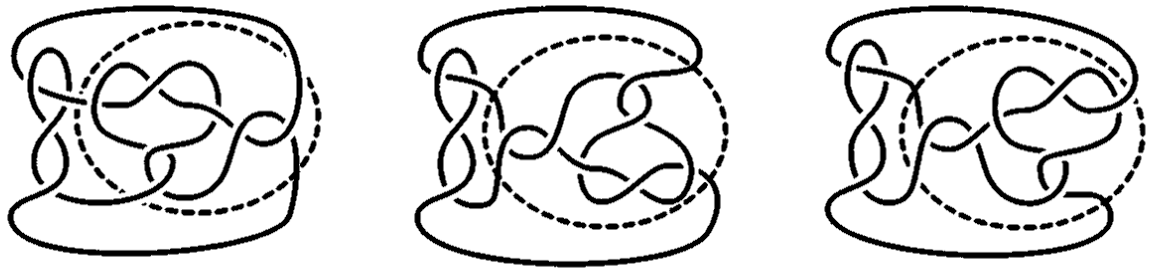
\includegraphics[width=0.7\linewidth]{cn13}
	\caption[Nudos mutantes entre sí]{Nudos mutantes entre sí}
	\label{fig:cn13}
\end{figure}

Uno de los nudos mutantes más conocidos son los llamados \textbf{mutantes de Kinoshita-Terasaka}.

\begin{figure}[ht]
	\centering
	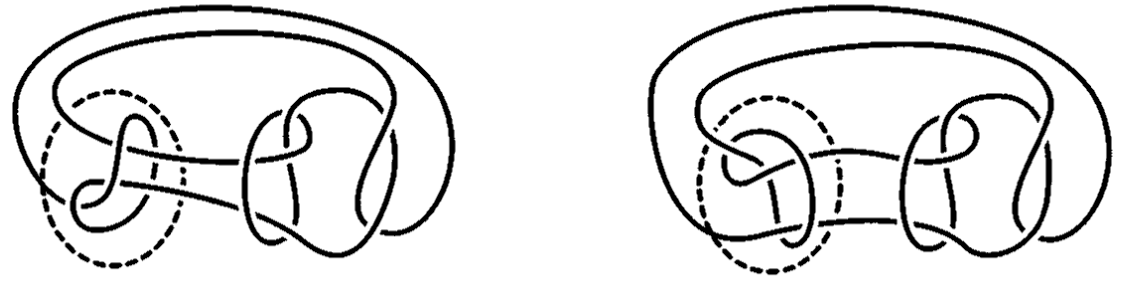
\includegraphics[width=0.7\linewidth]{cn14}
	\caption[Mutantes de Kinoshita-Terasaka]{Mutantes de Kinoshita-Terasaka}
	\label{fig:cn14}
\end{figure}

\chapter{Tipos de Nudos}
En el presente capítulo se estudiaran algunos conjuntos de nudos que comparten ciertas características, dividiéndolos dependiendo de sus características.

\section{Nudos Tóricos}
Los nudos tóricos no solo son interesantes por sí mismos, sino que también son importantes porque en muchas ocasiones ayudan a intuir propiedades generales de los nudos.

\begin{defn}\label{dfcp40} Diremos que un nudo es \textbf{tórico} si puede ser dibujado sin puntos de intersección en el toro.
\end{defn}

Existen diversas formas de poder construir nudos tóricos, explicaremos algunas de ellas. Para iniciar debemos notar que en el toro existen dos circunferencias estándar.

\begin{defn}\label{dfcp41} La circunferencia que recorre alrededor del toro de forma corta es conocida como \textbf{meridiano} y la que recorre alrededor del toro de forma larga es conocida como \textbf{longitud}.
\end{defn}

\begin{figure}[ht]
	\centering
	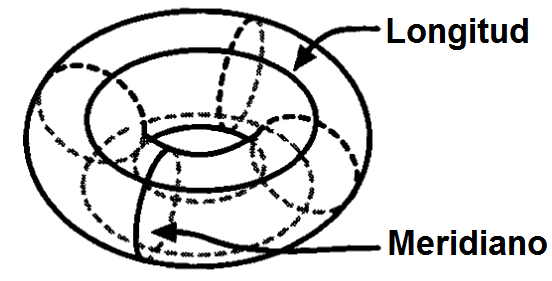
\includegraphics[width=0.4\linewidth]{t1}
	\caption[Meridianos y longitudes]{Meridianos y longitudes}
	\label{fig:t1}
\end{figure}

Una forma más formal de poder definir los conceptos anteriores es la siguiente: Recordemos que el conjunto $S^1\times S^1$ es homeomorfo a la superficie del toro, consideremos $f$ el homeomorfismo entre ambos conjuntos. Entonces tenemos que $f(e^{2\pi it},1)$ es un meridiano, mientras que $f(1,e^{2\pi it})$ es una longitud.

Entonces una forma para poder construir nudos tóricos es la siguiente: sean $m$ y $n$ un par de primos relativos. Definimos $K_{m,n}$ como el subconjunto del toro en $\mathbb{R}^3$
\[
K_{m,n}={f(e^{2\pi imt},e^{2\pi int})\mid t\in I}
\]

Donde $f$ es el homeomorfismo entre $S^1\times S^1$ y la superficie del toro, e $I=[0,1]$. Podemos ver que $g:S^1\rightarrow K_{m,n}$ definida por
\[
g(e^{2\pi it})=f(e^{2\pi imt},e^{2\pi int})
\]

Es un homeomorfismo del círculo en $K_{m,n}$ con lo cual $K_{m,n}$ es un nudo.

\begin{defn}\label{dfcp42} El nudo dado con anterioridad es conocido como \textbf{el nudo tórico de tipo $(m,n)$}.
\end{defn}

Una forma más intuitiva de ver un nudo tórico de tipo $(m,n)$ es decir que es un nudo tal que da $n$ vueltas alrededor del meridiano del toro y $m$ vueltas alrededor de la longitud del toro.

\begin{figure}[ht]
	\centering
	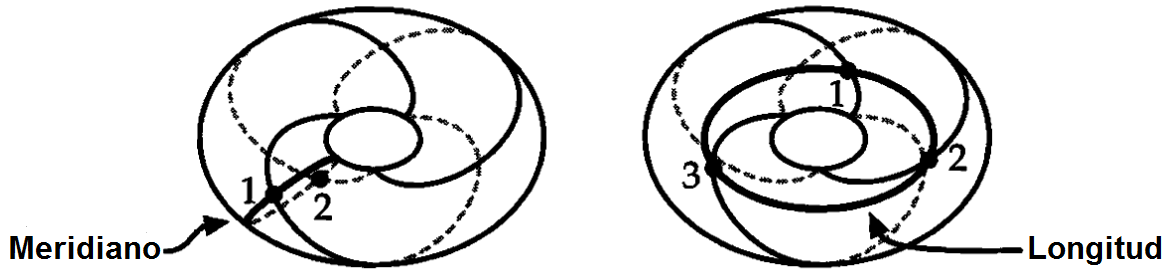
\includegraphics[width=0.7\linewidth]{t2}
	\caption[Nudo trébol como $(3,2)$-nudo tórico]{Nudo trébol como $(3,2)$-nudo tórico}
	\label{fig:t2}
\end{figure}

Supongamos que queremos dibujar el $(5,3)$-nudo tórico, debido a que dicho nudo debe dar cinco vueltas meridionales debería cruzar la longitud del toro cinco veces. Entonces marcamos cinco puntos en el ecuador exterior del toro y cinco puntos en el ecuador interior.

\begin{figure}[ht]
	\centering
	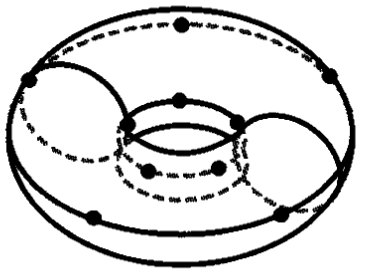
\includegraphics[width=0.25\linewidth]{t3}
	\caption[Puntos en el ecuador]{Puntos en el ecuador}
	\label{fig:t3}
\end{figure}

Queremos que el nudo de tres vueltas longitudinales, juntamos cada punto marcado en el ecuador exterior del toro con su correspondiente punto en el ecuador interior, utilizando un segmento que recorre el toro a través de la parte inferior.

\begin{figure}[ht]
	\centering
	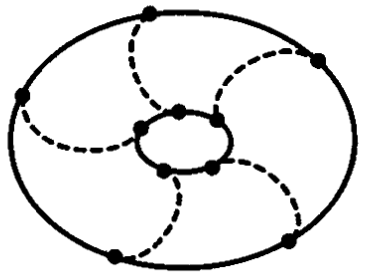
\includegraphics[width=0.25\linewidth]{t4}
	\caption{Uniendo puntos correspondientes}
	\label{fig:t4}
\end{figure}
\end{comment}
Ahora unimos cada punto en el ecuador exterior al punto en el ecuador interior que es el tercer punto a partir de la asignación anterior, recorriendo los puntos a favor de las manecillas del reloj.

\begin{figure}[ht]
	\centering
	\includegraphics[width=0.25\linewidth]{t5}
	\caption[$(5,3)$-nudo tórico]{$(5,3)$-nudo tórico}
	\label{fig:t5}
\end{figure}

Un procedimiento análogo se debe seguir para la construcción de un nudo tórico tipo $(p,q)$.

\begin{thm}\label{thm:t1} Cualquier $(p,q)$-nudo tórico es también un $(q,p)$-nudo tórico.
\end{thm}

\begin{proof}
	Consideremos un $(p,q)$-nudo tórico, removemos un pequeño disco del toro donde dicho nudo yace de tal forma que el disco no se intersecte con el nudo. Deformamos dicho toro con el disco removido en dos bandas que están unidas una con otra. La banda más corta corresponde al meridiano del toro, mientras que la banda más larga corresponde a la longitud del toro.
	
	Entonces tomamos la banda más larga y la giramos de adentro hacia afuera, luego realizamos el mismo procedimiento con la banda más pequeña. Entonces deformamos nuevamente las bandas para formar un nuevo toro con un disco removido pero con los roles de meridianos y longitudes cambiados, es decir, la banda que originalmente correspondía a la longitud ahora es la banda que corresponde al meridiano y la banda que originalmente correspondía al meridiano ahora es la banda que corresponde a la longitud. Debido a que la longitud y el meridiano intercambiaron papeles ahora tenemos un $(q,p)$-nudo tórico.
\end{proof}

Utilizando el $(3,2)$-nudo tórico ejemplificaremos la demostración anterior.

\begin{figure}[ht]
	\centering
	\includegraphics[width=0.8\linewidth]{t6}
	\caption[El $(3,2)$-nudo tórico es un $(2,3)$-nudo tórico]{El $(3,2)$-nudo tórico es un $(2,3)$-nudo tórico}
	\label{fig:t6}
\end{figure}

\begin{prp}\label{prp:t1}
	Todo $(p,q)$-nudo tórico siempre tiene una proyección con $p(q-1)$ cruces.
\end{prp}

\begin{proof}
	Consideremos un $(p,q)$-nudo tórico, construiremos una proyección que posea exactamente $p(q-1)$ cruces. Consideremos un cilindro con $q$ líneas dibujadas a lo largo de él, entonces manteniendo un lado fijo realizamos $p$ giros a favor de las manecillas del reloj obteniendo un el mismo cilindro pero ahora las líneas antes dibujadas se ven como espirales en él. Luego unimos los extremos del cilindro para formar así un toro. Entonces al proyectar dicho nudo en el plano y nos fijamos en alguna de las líneas antes dibujadas tenemos que dicha línea forma un ciclo en el cual pasa exactamente a través de las otras $q-1$ líneas restantes por cada giro dado, es decir se tienen $p(q-1)$ cruces. 
\end{proof}

Para ejemplificar el procedimiento anterior consideremos el $(4,3)$-nudo tórico, formaremos un nudo con $8$ cruces en su proyección.

\begin{figure}[ht]
	\centering
	\includegraphics[width=0.8\linewidth]{t7}
	\caption[Proyección de un nudo tórico]{Proyección de un nudo tórico}
	\label{fig:t7}
\end{figure}

Uniendo los dos resultados anteriores tenemos que un $(p,q)$-nudo tórico tiene una proyección con $p(q-1)$ cruces y una proyección con $q(p-1)$ cruces.

\begin{defn}\label{dfcp43} Llamaremos el \textbf{número de cruces} de un $(p,q)$-nudo tórico al mínimo entre $p(q-1)$ y $q(p-1)$.
\end{defn}

Podemos generalizar la noción de un nudo tórico. Por definición tenemos que un nudo tórico es un nudo no trivial que puede ser colocado en la superficie de un toro incrustado en $\mathbb{R}^3$ de forma estándar, sin que el nudo posea cruces en dicha superficie. Donde incrustado en $\mathbb{R}^3$ de forma estándar significa que el toro es no anudado en $\mathbb{R}^3$. Ciertamente, algunos nudos no pueden ser tóricos pero tal vez pueden ser colocados en superficies de otros géneros.

Tomemos por ejemplo una superficie de género dos, llamaremos un \textbf{nudo 2-incrustable} a un nudo que yace sin intersecciones en una superficie de género dos. Un ejemplo de ello es el nudo 8.

\begin{figure}[ht]
	\centering
	\includegraphics[width=0.35\linewidth]{t8}
	\caption[Nudo 2-incrustable]{Nudo 2-incrustable}
	\label{fig:t8}
\end{figure}

\section{Nudos Satélite}
Un segundo conjunto de nudos que se ha sido muy importante en los años recientes es el conjunto de los nudos satélite.

\begin{defn}\label{dfcp44} Sea $K_1$ un nudo dentro de un toro solido no anudado, con el toro formamos un segundo nudo $K_2$. Entonces el nudo $K_1$ que estaba dentro del toro original se transforma en un nuevo nudo dentro del toro anudado, a este nuevo nudo lo llamaremos un \textbf{nudo satélite}. El nudo $K_2$ es llamado el \textbf{nudo compañero} del nudo satélite.
\end{defn}

\begin{figure}[ht]
	\centering
	\includegraphics[width=0.25\linewidth]{s1}
	\caption[Un nudo $K_1$ dentro de un toro no anudado]{Un nudo $K_1$ dentro de un toro no anudado}
	\label{fig:s1}
\end{figure}

\begin{figure}[ht]
	\centering
	\includegraphics[width=0.4\linewidth]{s2}
	\caption[Toro anudado como $K_2$]{Toro anudado como $K_2$}
	\label{fig:s2}
\end{figure}

Siempre tomaremos un nudo no trivial como el nudo compañero, ya que de ser el nudo trivial tendríamos que el nudo satélite es el mismo nudo que el original. También vamos a asumir que el nudo $K_1$ toca a todos los discos meridionales del toro solido y no se puede saltar alguno de ellos. Pensamos en el nudo satélite como un nudo que permanece dentro de un toro solido que tiene un nudo compañero como su curva central, tal y como un satélite permanece en una órbita alrededor del planeta.

Si tomamos el nudo original $K_1$ como un no nudo pero con un giro, entonces el nudo satélite resultante es llamado un \textbf{Whitehead doble} del nudo compañero. El nombre hace referencia al hecho que $K_1$ se asemeja al enlace de Whitehead.

\begin{figure}[ht]
	\centering
	\includegraphics[width=0.4\linewidth]{s3}
	\caption[El Whitehead doble del nudo trébol]{El Whitehead doble del nudo trébol}
	\label{fig:s3}
\end{figure}

Un Whitehead doble no es único. Podemos cortar el toro solido a lo largo de un disco meridional, girar un extremo algún número de veces y entonces pegamos nuevamente los discos para obtener una copia homeomorfa del toro solido pero ahora dos hilos de $K_1$ están enrollados entre ellos. Entonces cuando el anudamos el toro sólido como el nudo trébol obtenemos un segundo Whitehead doble del nudo trébol. 

\begin{figure}[ht]
	\centering
	\includegraphics[width=0.235\linewidth]{s4}
	\caption[Un segundo Whitehead doble del nudo trébol]{Un segundo Whitehead doble del nudo trébol}
	\label{fig:s4}
\end{figure}

Si el nudo origina $K_1$ es nuevamente un no nudo, pero ahora como en la figura~\ref{fig:s5}, entonces el nudo satélite resultante es llamado un \textbf{cable de dos hilos} del nudo compañero. Es como si tuviéramos un cable que recorre dos veces el nudo compañero. Nuevamente el cable de dos hilos de un nudo acompañante no es único, podríamos realizar un procedimiento como para los Whitehead dobles.

\begin{figure}[ht]
	\centering
	\includegraphics[width=0.55\linewidth]{s5}
	\caption[Cable de dos hilos del nudo trébol]{Cable de dos hilo del nudo trébol}
	\label{fig:s5}
\end{figure}

      % Cap. 1 

%\include{tch2}      % Cap. 2 

%\include{tch3}      % Cap. 3 
{\backmatter     %	Capítulos no van numerados --------------------------------------------------  Apartados finales
\begin{comment}
%%% INCLUYA SUS CONCLUSIONES Y RECOMENDACIONES


\chapter{CONCLUSIONES}
\begin{enumerate}
	\item Conclusión 1.
	\item Conclusión 2.
	\item Conclusión 3.
\end{enumerate}

\chapter{RECOMENDACIONES}
\begin{enumerate}
	\item Recomendación 1.
	\item Recomendación 2.
	\item Recomendación 3.
\end{enumerate}
     % Conclusiones y recomendaciones


\begin{thebibliography}{99}
%% La bibliografía se ordena en orden alfabético respecto al apellido del 
%% autor o autor principal
%% cada entrada tiene su formatado dependiendo si es libro, artículo,
%% tesis, contenido en la web, etc

% artículo en una revista arbitrada
\bibitem{albin} P. Albin, E. Leichtnam, R. Mazzeo y P. Piazza. The signature package on Witt spaces. \textit{Ann. Sci. Ec. Norm. Supér. (4)}, \textbf{45}(2):241--310, 2012.

% libro
\bibitem{Brez} H. Brezis. \textit{Analyse functionnelle, théorie et applications.} (Collection Mathématiques Appliquées pour la Maítrise) Masson, Paris, 1992.

% libro
\bibitem{Choq} Y. Choquet"=Bruhat y otros. \textit{Analysis, manifolds and physics. (volumen 1)} North"=Holland Publishing Company, Amsterdam, 1996.

% libro
\bibitem{C:H2} R. Courant y {D. Hilbert}. \textit{Methods of mathematical physics. (volumen 2)} Interscience Publishers, Nueva York, 1962.

% artículo en la web arXiv, preprint
\bibitem{Rafa4} R. {De la Madrid}. The rigged {Hilbert} space of the free hamiltonian. Consultado en marzo de 2005 en \url{http://arxiv.org/abs/quant-ph/0210167}.

% libro con datos faltantes, s.e. "sin editorial"
\bibitem{Doc} J. Escamilla-Castillo. \textit{Topología.} 2"a ed. s.e., Guatemala, 1992.

% libro traducido
\bibitem{Hasr} N. Haaser y {J. Sullivan}. \textit{Análisis real.}  Tr.~Ricardo Vinós. Trillas, México, 1978.

% libro traducido
\bibitem{Halmo} P. Halmos. \textit{Teoría intuitiva de los conjuntos.} 8"a ed. Tr.~Antonio Martín. Compañía Editorial Continental, S.A., México, 1973.

% libro 
\bibitem{Haus} F. Hausdorff. \textit{Set theory.} 2"a ed. Chelsea Publishing Company, Nueva York, 1962.

% libro
\bibitem{Heis} W. Heisenberg. \textit{The physical principles of the quantum theory.} Dover Publications, Inc., Nueva York, 1949.

% libro
\bibitem{Hewit} E. Hewitt y {K. Stromberg}. \textit{Real and abstract analysis.} Springer"=Verlag, Nueva York, 1965.

% libro
\bibitem{Kolmo} A. Kolmogorov y {S. Fomin}. \textit{Elementos de la teoría de funciones y del análisis funcional.} Tr.~Carlos Vega. MIR, Moscú, 1975.

% artículo de una enciclopedia en línea
\bibitem{Kronz} F. Kronz. Quantum theory: von {Neumann} versus {Dirac}. Consultado en marzo de 2005 en \url{http://plato.stanford.edu/entries/qt-nvd/}.

% artículo en una revista arbitrada
\bibitem{liu} K. Liu, X. Sun, and S.-T. Yau. Goodness of canonical metrics on the moduli space of Riemann surfaces. \textit{Pure Appl. Math. Q.}, \textbf{10}(2):223--243, 2014

% artículo en una revista arbitrada
\bibitem{leader} E. Leader and C. Lorcé, The angular momentum controversy: What's it all about and does it matter?, \textit{Phys. Rept.} \textbf{541}, 163 (2014).

% libro
\bibitem{Omnes} Omn\`{e}s, R. \textit{The interpretation of quantum mechanics.} (Princeton Series in Physics) Princeton University Press, Princeton, 1994.

% libro
\bibitem{Penr} R. Penrose. \textit{La mente nueva del emperador.} Tr.~José García. Fondo de Cultura Económica, México, 1996.

% publicación electrónica
\bibitem{Ster} S. Sternberg. Theory of functions of a real variable. Consultado en abril de 2005 en \url{http://www.math.harvard.edu/\~shlomo}.

% publicación electrónica
\bibitem{Tesc} G. Teschl. Mathematical methods in quantum mechanics with applications to {Schrödinger} operators. Consultado en abril de 2005 en \url{http://www.mat.univie.ac.at/\~gerald}.

\end{thebibliography}
   % Bibliografía
}

% Descomentar en el caso de necesitar incluir apéndices
%\appendix			% Apéndices

%\begin{comment}
\chapter{CONCEPTOS BÁSICOS DE TEORÍA DE NUDOS}
En el presente capítulo se presentan las definiciones y teoremas básicos en el estudio de la teoría de nudos. Se realizan las demostraciones que son cruciales para el contenido a desarrollar más adelante.

\section{Nudos y enlaces}
\subsection{Nudos}
Para el estudio matemático de lo que físicamente se comprende como un nudo se requiere plantear una definición matemática de nudo que concuerde con el modelo físico. Así la definición formal de un nudo es la siguiente:

\begin{defn}\label{dfcp1} El subconjunto $K\subset\mathbb{R}^3$ es un \textbf{nudo} si existe un homeomorfismo del círculo unitario $S^1$ en $\mathbb{R}^3$ cuya imagen es $K$.
\end{defn}

El ejemplo más simple de un nudo es la circunferencia $S^1$ vista en $\mathbb{R}^3$, este nudo es conocido como \textbf{no nudo} o \textbf{nudo trivial}, figura~\ref{fig:nudotrivial}, además otro ejemplo de un nudo simple es el \textbf{nudo trébol}, figura~\ref{fig:nudotrebol}.

\begin{figure}[ht]
	\centering
	\includegraphics[width=0.175\linewidth]{trebol}\\
	\caption[Nudo Trébol]{Nudo Trébol}
	\label{fig:nudotrebol}
\end{figure}

\begin{figure}[ht]
	\centering
	\includegraphics[width=0.175\linewidth]{Trivial}\\
	\caption[Nudo Trivial]{No Nudo o Nudo trivial}
	\label{fig:nudotrivial}
\end{figure}

El primer interrogante que surge al hablar sobre el nudo trivial y el nudo trébol es: ¿cómo saber que efectivamente estos dos nudos son distintos? Para resolver a esta pregunta primero se debe definir cuando dos nudos son el mismo nudo.

\begin{defn}\label{dfcp2} Sean $K_1$, $K_2$ dos nudos, diremos que son \textbf{equivalentes} o el mismo nudo si existe una función continua $H:\mathbb{R}^3\times[0,1]\rightarrow\mathbb{R}^3$ tal que $H(K_0,0)~=~K_0$, $H(K_0,1)=K_1$ y además $H$ es inyectiva en el intervalo $[0,1]$. $H$ es llamada una \textit{isotopía espacial} de $K_1$ en $K_2$.
\end{defn}

Esto quiere decir que dos nudos son equivalentes si podemos transformar uno en el otro de forma continua, es decir, sin romper el nudo original. Denotaremos como $K_1\simeq K_2$ al hecho que $K_1$ sea equivalente a $K_2$.

Existen varias formas de poder visualizar a los nudos para su estudio, una de ellas es ver a un nudo como una función parametrizada en $\mathbb{R}^3$, es decir, $f(t)=(x(t),y(t),z(t))$ donde $0<t<1$ y $f(0)=f(1)$. Esta forma de ver a un nudo es útil si se tiene algún interés en su posición en el espacio\footnote{La posición del nudo en el espacio es un tema de interés en la teoría de nudos geométrica.}, pero para la teoría a estudiar más adelante es conveniente olvidarnos de la posición del nudo en el espacio. Es por ello que definimos el diagrama de un nudo.

\begin{defn}\label{dfcp3} Un \textbf{diagrama de nudo} es la proyección del nudo en $\mathbb{R}^2$.
\end{defn}

Aunque el nudo original no posea auto-intersecciones al proyectar dicho nudo en el plano si pueden aparecer auto-intersecciones, por ello indicamos cual hebra pasa por arriba y cual por abajo dibujando de forma discontinua la hebra que pasa por abajo y de forma continua la hebra que pasa por arriba.

\begin{defn}\label{dfcp4} Un \textbf{cruce} es el punto donde el diagrama de nudo tiene una auto-intersección.
\end{defn}

Por ejemplo el nudo trivial tiene 0 cruces mientras que el nudo trébol posee 3 cruces.

\begin{defn}\label{dfcp5} Un nudo es llamado \textbf{dócil} si su diagrama posee una cantidad finita de cruces. En caso contrario es llamado \textbf{nudo salvaje}.
\end{defn}

Para la simplificación de la teoría en ocasiones, es conveniente, trabajar con un tipo particular de nudo y luego generalizarlo. Uno de los tipos más interesantes y útiles de nudos es el nudo alternante.

\begin{defn}\label{dfcp6} Un nudo es llamado \textbf{alternante} si en su diagrama las hebras van alternando entre arriba y abajo al recorrer el nudo en una dirección fija.
\end{defn}

Al igual que muchos de los objetos matemáticos los nudos pueden operarse entre ellos para formar un nuevo nudo.

\begin{defn}\label{dfpc7} Dados dos diagramas de nudos, removemos un pequeño arco de cada diagrama y conectamos los cuatro puntos finales, a pares, con nuevos arcos formando un nuevo nudo, este nuevo nudo es conocido como la \textbf{composición} de los nudos iniciales. Si tenemos dos nudos $J$ y $K$ su composición la denotamos como $J\# K$
\end{defn}

\begin{figure}[ht]
	\centering
	\includegraphics[width=0.8\linewidth]{ncomposicion}\\
	\caption[Composición de nudos]{Composición de nudos}
	\label{fig:composición}
\end{figure}

Para la formación de un nudo compuesto hay algunos consideraciones a tomar en cuenta: los nudos con los cuales se desea realizar la composición no deben estar superpuestos, los arcos que se eligen para remover no deben afectar los cruces del nudo original y los arcos introducidos para formar el nuevo nudo no deben formar nuevos cruces con el nudo original. 

\begin{figure}[ht]
	\centering
	\includegraphics[width=0.4\linewidth]{nnocom}\\
	\caption[Ejemplo de como no se realiza la composición de nudos]{Ejemplo de como no se realiza la composición de nudos}
	\label{fig:nocom}
\end{figure}	

\begin{defn}\label{dfcp8} Un nudo es llamado \textbf{compuesto} si puede ser expresado como la composición de dos nudos, donde ninguno de los nudos por los cuales está formado son el nudo trivial y los nudos por los cuales está formado son llamados \textbf{nudos factor}. 
\end{defn}

El pedir que ninguno de los nudos factor sea el nudo trivial es porque el nudo trivial bajo la composición de nudos es el análogo al $0$ en los reales bajo la suma, es decir, si denotamos al nudo trivial como $K$ y tomamos un nudo cualesquiera $J$ tendríamos $J\# K=K\# J=J$. Entonces esto indicaría que cualquier nudo es un nudo compuesto.

\begin{figure}[ht]
	\centering
	\includegraphics[width=0.6\linewidth]{ncomtriv}\\
	\caption[composición de un nudo con el nudo trivial]{Composición con el nudo trivial}
	\label{fig:comtriv}
\end{figure}

\begin{defn}\label{dfcp9} Un nudo que no es composición de cualesquiera dos nudos no triviales es llamado \textbf{nudo primo}.
\end{defn}

Para el trabajo con nudos compuestos es necesario resolver la siguiente pregunta ¿El nudo trivial es compuesto? En la figura \ref{fig:nudotrivial} podríamos pensar que no es un nudo compuesto, pero tal vez existe otra forma de proyectar el nudo trivial que contradiga esto.

\begin{prp}\label{prop1} El nudo trivial es un nudo primo.
\end{prp}

\begin{proof} Supongamos que el nudo trivial es un nudo compuesto, es decir, es la composición de por lo menos dos nudos distintos del nudo trivial. Sabemos que podemos pensar en cualquier nudo como la composición del nudo trivial con el mismo nudo, entonces como estamos suponiendo que el nudo trivial es compuesto tenemos que cualquier nudo puede ser visto como la composición de él mismo con los componentes del nudo trivial y esto implicaría que cualquier nudo es compuesto, lo cual es imposible.
\end{proof}

Este resultado es análogo a pensar en el $1$ en los naturales con el producto, es decir, la única forma de realizar la composición de dos nudos y esta nos regrese el nudo trivial es que los nudos con los que se realiza la composición son equivalentes al nudo trivial.

Pero a diferencia de los números naturales donde el orden de los factores no altera el producto, en la composición de nudos es posible poder formar distintos nudos compuestos del mismo par de nudos. Esto es posible al elegir distintos arcos que suprimir o darle otra orientación al nudo.

\begin{defn}\label{dfcp10} Una \textbf{orientación} es una elección para viajar a través del diagrama del nudo. Esta dirección es denotada en el diagrama por flechas. A un nudo provisto de una orientación le llamaremos \textbf{nudo orientado}.
\end{defn}

\begin{figure}[ht]
	\centering
	\includegraphics[width=0.3\linewidth]{orientado}\\
	\caption[Nudo trébol orientado]{Nudo trébol orientado}
	\label{fig:orientado}
\end{figure}

Entonces para cualesquiera par de nudos orientados $J$ y $K$, existen dos posibilidades de composición: La orientación sobre $J$ coincide con la orientación sobre $K$ en $J\#K$, resultando en una orientación para $J\#K$; o la orientación sobre $J$ y sobre $K$ no coinciden en $J\# K$. Todas las composiciones de dos nudos cuya orientación coincide producen el mismo nudo, análogamente para las composiciones cuya orientación no coincide.

\begin{figure}[ht]
	\centering
	\includegraphics[width=0.3\linewidth]{ncoinciden}\\
	\caption[Composición de dos nudos cuyas orientaciones coinciden]{Composición de dos nudos cuyas orientaciones coinciden}
	\label{fig:coinciden}
\end{figure}

\begin{figure}[ht]
	\centering
	\includegraphics[width=0.35\linewidth]{nnocoinciden}\\
	\caption[Composición de dos nudos cuyas orientaciones no coinciden]{Composición de dos nudos cuyas orientaciones no coinciden}
	\label{fig:nocoinciden}
\end{figure}

Es posible que los nudos compuestos cuyas orientaciones coinciden sean los mismos que los nudos compuestos cuyas orientaciones no coinciden, para ello es necesario el concepto de nudo invertible.

\begin{defn}\label{dfcp11} Diremos que un nudo orientado es \textbf{invertible} si es equivalente a sí mismo pero con la orientación en sentido contrario.
\end{defn}

Si realizamos la composición de un nudo orientado invertible con un nudo orientado cualesquiera tendríamos que su composición cuando la orientación concuerda y cuando la orientación no concuerda es la misma.

\begin{defn}\label{dfcp28} El \textbf{anverso} de un nudo $K$ es la imagen de espejo de $K$ y es denotado por $\overline{K}$.
\end{defn}

Un nudo cualesquiera puede o no ser equivalente a su anverso.

\begin{defn}\label{dfcp29} Un nudo que es equivalente a su anverso es llamado \textbf{anfiquiral}\footnote{El termino anfiquiral es comúnmente usado por matemáticos, pero algunos químicos suelen usar el termino \textbf{aquiral} en referencia a lo mismo.}.
\end{defn}

Un ejemplo de un nudo que no es anfiquiral es el nudo trébol debido a que no es equivalente a su anverso, figura~\ref{fig:chiral}.

\begin{figure}[ht]
	\centering
	\includegraphics[width=0.5\linewidth]{chiral}\\
	\caption[Nudo no anfiquiral]{Nudo no anfiquiral}
	\label{fig:chiral}
\end{figure}

La prueba de que efectivamente este nudo no es anfiquiral la realizaremos más adelante.

\subsection{Enlaces}
Hasta el momento hemos restringido nuestra atención a los nudos, que puede ser visto como un lazo anudado, es decir, una cuerda entrelazada consigo misma y unida en sus extremos. Pero no hay razones para decir que se puede trabajar con un solo lazo.

\begin{defn}\label{dfcp12} Un \textbf{enlace} es una colección finita de nudos posiblemente enlazados entre sí. Análogo a lo conocido para nudos decimos que dos enlaces son el mismo o son \textbf{equivalentes} si podemos deformar uno en el otro de manera continua.
\end{defn}

Algunos ejemplos de enlaces simples conocidos son los llamados \textbf{enlaces de Whitehead}, figura~\ref{fig:whitehead}. Estos enlaces están formados por dos bucles anudados.

\begin{figure}[ht]
	\centering
	\includegraphics[width=0.5\linewidth]{nwhitehead}\\
	\caption[Enlaces de Whitehead]{Enlaces de Whitehead}
	\label{fig:whitehead}
\end{figure}

\begin{defn}\label{dfcp13} Llamaremos \textbf{componente} de un enlace a cada bucle anudado (nudo) del cual esta formado el enlace.
\end{defn}

Podríamos considerar un nudo como un enlace de un solo componente. Dado que los enlaces de Whitehead están hechos de dos bucles anudados diremos que es un enlace con dos componentes. Otro ejemplo de enlace simple son llamados \textbf{anillos de Borromeo}.

\begin{figure}[ht]
	\centering
	\includegraphics[width=0.2\linewidth]{borromean}\\
	\caption[Anillos de Borromeo]{Anillos de Borromeo}
	\label{fig:borromean}
\end{figure}

\begin{defn}\label{dfcp14} Un enlace es llamado \textbf{dividible} si los componentes del enlace pueden ser deformados de modo que se encuentren en diferentes lados del plano en el espacio tridimensional. 
\end{defn}

Existe una forma rápida de decir que dos enlaces no son el mismo, simplemente verificando el número de componentes que poseen. Pero no siempre trabajaremos con enlaces con diferente número de componentes, estamos interesados en saber cuando dos enlaces de igual número de componentes son distintos.

Un ejemplo inicial está dado por los enlaces más simples de dos componentes, el primero conocido como \textbf{enlace trivial} y el segundo \textbf{enlace de Hopf}, figura~\ref{fig:enlacetrivial}. Estos enlaces difieren el uno del otro debido a que el primero es dividible mientras que el segundo no.

\begin{figure}[ht]
	\centering
	\includegraphics[width=0.55\linewidth]{enlacetrivial}\\
	\caption[Enlace trivial y enlace de Hopf]{Enlace trivial y enlace de Hopf}
	\label{fig:enlacetrivial}
\end{figure}

Sean $M$ y $N$ dos componentes en un enlace y elegimos una orientación en cada uno de ellos. Entonces a cada cruce entre las dos componentes se le puede asignar un $+1$ o un $-1$ dependiendo del caso (figura \ref{fig:numero}).

\begin{figure}[ht]
	\centering
	\includegraphics[width=0.35\linewidth]{numero}\\
	\caption[Enlaces]{Enlaces}
	\label{fig:numero}
\end{figure}

En la figura~\ref{fig:numero}, si tenemos un cruce del primer tipo (izquierda) se le asigna un $-1$ mientras que para el segundo tipo (derecha) se le asigna un $+1$.

\begin{defn}\label{dfcp15} Sea $L$ un enlace orientado y sea $M$ el conjunto de todos los cruces en $L$ con su respectivo valor, entonces el \textbf{número de enlace} de $L$ es la suma de todos los valores de los cruces en $M$ dividido entre 2.
\end{defn}

Por ejemplo el enlace trivial tiene número de enlace 0, el  enlace Hopf tiene número de enlace 1 o -1 dependiendo de la orientación. Otro ejemplo es el mostrado en la figura \ref{fig:linking}.

\begin{figure}[ht]
	\centering
	\includegraphics[width=0.2\linewidth]{nlinking}\\
	\caption[Número de enlace]{Número de enlace 2}
	\label{fig:linking}
\end{figure}

\begin{defn}\label{dfcp16} Un enlace es llamado \textbf{alternante} si en su diagrama las hebras van alternando entre arriba y abajo al recorrer el nudo en una dirección fija.
\end{defn}

Notemos que esta definición es análoga a la de nudo alternante, y así como esta algunas definiciones o teoremas son similares tanto en nudos como en enlaces.
\end{comment}
\begin{comment}
\section{Movimientos de Reidemeister}
Uno de los grandes problemas en la teoría de nudos es el clasificar los nudos, es decir, saber cuando un nudo es distinto a otro. En la sección anterior se habló brevemente de la equivalencia de nudos, pero trataremos de manera formal las definiciones antes dadas.

\begin{defn}\label{dfcp17} Sean $X$ y $Y$ espacios de Hausdorff. Una función $f:X\rightarrow Y$ es llamada una \textbf{incrustación} si $f:X\rightarrow f(X)$ es un homeomorfismo.
\end{defn}

\begin{defn}\label{dfcp18} Dos incrustaciones $f_0,f_1:X\rightarrow Y$ son \textbf{isotópicas} si existe una incrustación $F:X\times I \rightarrow Y\times I$ tal que $F(x,t)=(F(x,t),)$, $x\in X$, $t\in I=[0,1]$ con $f(x,0)=f_0(x)$, $f(x,1)=f_1(x)$. F es llamada \textbf{isotopía de conservación de nivel} o simplemente \textbf{isotopía}.
\end{defn}

Usaremos con frecuencia la notación $f_t(x)=f(x,t)$. Esta noción de isotopía no es buena en temas relacionados con los nudos, es por ello que necesitamos la siguiente definición:

\begin{defn}\label{dfcp19} Dos incrustaciones $f_0,f_1:X\rightarrow Y$ son \textbf{isotópicas en el espacio} si existe una isotopía $H:X\times I \rightarrow Y\times I$, $H(y,t)=(h_t(y),t)$, con $f_1=h_1f_0$ y $h_0=id_Y$. La función H es llamada un \textbf{isotopía espacial}.
\end{defn}

Una isotopía espacial define una isotopía $F$ que conecta $f_0$ con $f_1$ por $F(x,t)=(h_tf_0(x),t)$. La diferencia entre las dos definiciones anteriores es la siguiente: una isotopía transforma continuamente el conjunto $f_0(X)$ en $f_1(X)$ en Y, pero no toma en cuenta los puntos de $Y$ fuera de $f_1(X)$. Una isotopía espacial requiere que $Y$ se mueva continuamente junto con $f_t(X)$.

\begin{defn}\label{dfcp20} La \textbf{representación poligonal} de un nudo es la unión de los segmentos $[p_1,p_2],[p_2,p_3],...,[p_{n-1},p_n],[p_n,p_1]$ de un conjunto ordenado de distintos puntos $(p_1,p_2,...,p_n)$ formando el nudo.
\end{defn}

\begin{figure}[ht]
	\centering
	\includegraphics[width=0.3\linewidth]{poligonal}\\
	\caption[Representación poligonal del nudo trébol]{Representación poligonal del nudo trébol}
	\label{fig:poligonal}
\end{figure}

En ocasiones trabajaremos con la forma poligonal de un nudo, para ello utilizaremos la categoría p.l.\footnote{p.l. viene del inglés \textit{piecewise linear}} Los conceptos de isotopía e isotopía espacial son análogos a las definiciones anteriores para la categoría p.l.

\begin{defn}\label{dfcp22} Dos nudos (p.l.-nudos) son \textbf{equivalentes} si son isotópicos en el espacio (p.l.-isotópicos en el espacio).
\end{defn}

Los conceptos anteriores no son prácticos al trabajar, es por ello que trabajaremos dichos conceptos a través de movimientos en el espacio y en el plano.

\begin{defn}\label{dfcp23} Sea $u$ un segmento de un nudo poligonal $K$ en $\mathbb{R}^3$ y $D$ un triángulo en $\mathbb{R}^3$, $\partial D=u\cup v\cup w$, es decir, los lados de $D$ son $u$, $v$, $w$. Si $D\cap K=u$, entonces $K'=(K-u)\cup v\cup w$ define otro nudo poligonal. Diremos que $K'$ resulta de $K$ por un \textbf{$\Delta-$proceso} o un \textbf{$\Delta-$movimiento}. Si $K$ es orientado, $K'$ tiene que llevar la orientación inducida por $K$. El proceso inverso es denotado por $\Delta^{-1}$.
\end{defn}

\begin{figure}[ht]
	\centering
	\includegraphics[width=0.6\linewidth]{tmov}\\
	\caption[$\Delta-$movimiento]{$\Delta-$movimiento}
	\label{fig:tmov}
\end{figure}

\begin{defn}\label{dfcp24} Dos nudos son \textbf{combinatóricamente equivalentes} o \textbf{isotópicos por movimientos}, si existe una sucesión finita de $\Delta-$movimientos o $\Delta^{-1}-$movimientos que transforma un nudo en el otro.
\end{defn}

Ya que tenemos distintas definiciones de equivalencia de nudos es necesario demostrar que estas definiciones son equivalentes. Para esto son necesarios algunos teoremas previos:

\begin{thm}\label{thm:schoenflies} (Alexander-Schoenflies) Sea $i:S^2\rightarrow S^3$ una incrustación (p.l.-incrustación). Entonces
	\begin{equation*}
		S^3=B_1\cup B_2,\text{ }  i(S^2)=B_1\cap B_2=\partial B_1=\partial B_2	
	\end{equation*}
donde $B_i$, $i=1,2$, es una 3-bola combinatórica ($B_i$ es p.l.-homeomorfa a un 3-tetraedro)
\end{thm}

%demostración pendiente, aún no la encuentro.

Este teorema corresponde al teorema de la curva de Jordan en dos dimensiones.

\begin{prp}\label{prp:Tietze} (Alexander-Tietze) Cualquier homeomorfismo (p.l.-homeomorfismo) $f$ de una n-bola $B$ que mantiene la frontera fija es isotópico a la identidad por una isotopía espacial (p.l.-isotopía espacial) que mantiene fija la frontera.
\end{prp}
%copia literal de la demostración, detalles pendientes
\begin{proof} 
	Definamos para $(x,t)\in \partial(B\times I)$ la siguiente función:
	\begin{equation*}
		H(x,t)=\left\{\begin{array}{lcc}
			x & si & t=0\\
			x & si & x\in\partial B\\
			f(x) & si & t=1
		\end{array}
		\right.
	\end{equation*}
	Cualquier punto $(x,t)\in B\times I$, $t>0$ está en un segmento recto en $B\times I$ uniendo un punto interior fijo $P$ de $B\times 0$ y un punto variable $X$ en $\partial(B\times I)$. Extendemos $H\mid\partial(B\times I)$ linealmente a lo largo de estos segmentos obteniendo un isotopía $H:B\times I\rightarrow B\times I$, en efecto, la isotopía espacial deseada. %colocar referencia
\end{proof}

\begin{figure}[ht]
	\centering
	\includegraphics[width=0.3\linewidth]{tietze}\\
	\caption[Proposición de Alexander-Tietze]{Proposición de Alexander-Tietze}
	\label{fig:tietze}
\end{figure}

\begin{prp}\label{prp:equivalencia}
	Sean $K_0$, $K_1$ nudos (p.l.-nudos) en $S^3$ los siguientes enunciados son equivalentes:
	\begin{enumerate}
		\item Existe un homeomorfismo que preserva la orientación $f:S^3\rightarrow S^3$ que transforma $K_0$ en $K_1$, $f(K_0)=K_1$.
		\item $K_0$ y $K_1$ son equivalentes (isotópicos en el espacio).
		\item $K_0$ y $K_1$ son combinatóricamente equivalentes (isotópicos por movimientos).
	\end{enumerate}
\end{prp}

\begin{proof}
	$(1)\Rightarrow(2)$ Iniciaremos probando que existe una isotopía espacial $H(x,t)=(h_t(x),t)$ de $S^3$ tal que $h_1f$ deja fijo un 3-tetraedro $[P_0,P_1,P_2,P_3]$. Si $f:S^3\rightarrow S^3$ tiene un punto fijo, elijamos es te punto como $P_0$; sino, sea $P_0$ cualquier punto interior de un 3-tetraedro $[s^3]$ de $S^3$. Existe una isotopía espacial de $S^3$ que deja $\overline{S^3-[s^3]}$ fijo y lleva $P_0$ a cualquier otro punto interior de $[s^3]$. Si $[s^3]$ y $[s'^3]$ tienen una cara común, uno puede fácilmente construir una isotopía espacial que mueva un punto interior $P_0$ de $[s^3]$ a un punto interior $P_0'$ de $[s'^3]$ que es la identidad fuera de $[s^3]\cup[s'^3]$, figura~\ref{fig:equivalencia}.
	\begin{figure}[ht]
	\centering
	\includegraphics[width=0.4\linewidth]{equivalencia}\\
	\caption[Construcción de isotopía]{Construcción de isotopía}
	\label{fig:equivalencia}
	\end{figure}
	Así existe una isotopía espacial $H^0$ con $h_1^0f(P_0)=P_0$, desde que cualesquiera dos 3-tetraedros pueden ser conectados por una cadena de \textit{adjoining ones}. Luego elijamos un punto $P_1\neq P_0$ en el tetraedro de $P_0$, y por argumentos similares construimos una isotopía espacial $H_1$ con $h_1^1h_1^0f$ que deja fijo al 1-tetraedro $[P_0,P_1]$. Un paso más conduce a $h_1^2h_1^1h_1^0f$ con un 2-tetraedro $[P_0,P_1,P_2]$ fijo. En este momento la suposición viene en que f es necesario para preservar la orientación. Un punto $P_3\not\in [P_0,P_1,P_2]$, pero en la estrella de $[P_0,P_1,P_2]$, sería mapeado por $h_1^2h_1^1h_1^0f$ en un punto $P'^3$ en el mismo medio espacio con respecto al plano generado por $P_0$, $P_1$, $P_2$. Esto asegura la existencia de una isotopía espacial final $H^3$ tal que $h_1^3h_1^2h_1^1h_1^0f$ mantiene $[P_0,P_1,P_2,P_3]$ fijo. Esta afirmación se sigue del hecho que $H=H^3H^3H^1H^0$ es una isotopía espacial, $H(x,t)=(h_t(x),t)$. Por el teorema~\ref{thm:schoenflies} el complemento de $[P_0,P_1,P_2,P_3]$ es una 3-bola combinatórica y por la proposición~\ref{prp:Tietze} hay una isotopía espacial que conecta $h_1f$ con la identidad de $S^3$.
	
	$(2)\Rightarrow(1)$ consecuencia directa de la definición de isotopía espacial.
	
	$(1)\Rightarrow(3)$ Sean $K_0$ y $K_1$ nudos y sea $h:S^3\rightarrow S^3$ un homeomorfismo que preserva la orientación tal que $K_1=h(k_0)$. El argumento anterior muestra que hay otro homeomorfismo que preserva la orientación, $g:S^3\rightarrow S^3$ con $g(K_0)=K_0$, tal que $hg$ deja fijo algún 3-tetraedro $[s^3]$ que tendrá que ser elegido fuera de una vecindad regular de $K_0$ y $K_1$. Para un punto interior $P$ de $[s^3]$ consideremos $S^3-{P}$ como $\mathbb{R}^3$. Hay una traslación $\tau$ de $\mathbb{R}^3$, que mueve $K_0$ en $[s^3]-{P}$. Es fácil probar que $K_0$ y $\tau(K_0)$ son isotópicos por movimientos, figura~\ref{fig:equivalencia2}. Afirmamos que $K_1=hg(K_0)$ y $hg\tau(K_0)=\tau(K_0)$ son isotópicos por movimientos, que completaría la prueba: elijamos una subdivisión de la tiangulación de $S^3$ tal que los triángulos usados en la isotopía por movimientos entre $K_0$ y $\tau(K_0)$ forman un \textit{subcomplex} de $S^3$. Hay una isotopía por movimientos tal que $K_0\rightarrow\tau(K_0)$ que esta definida en los triángulos de la subdivisión. $hg:S^3\rightarrow S^3$ mapea el \textit{subcomplex} en otro que lleva la isotopía por movimientos.
	\begin{figure}[ht]
		\centering
		\includegraphics[width=0.4\linewidth]{equivalencia2}\\
		\caption[Isotopía por movimientos $K_0\rightarrow\tau(K_0)$]{Isotopía por movimientos $K_0\rightarrow\tau(K_0)$}
		\label{fig:equivalencia2}
	\end{figure}

	$(3)\Rightarrow(1)$ No es difícil de construir un homeomorfismo de $S^3$ en si mismo que realice un $\Delta^{\pm1}$-movimiento y deje fijo el resto del nudo. Elijamos una vecindad regular $U$ de un 2-tetraedro que define el $\Delta^{\pm1}$-movimiento cuya frontera coincide con el nudo en dos puntos. Por extensión lineal uno puede obtener un homeomorfismo que produzca el $\Delta^{\pm1}$-movimiento en $U$ y deje $S^3-U$ fijo.
\end{proof}

La descripción geometrica en el espacio tridimensional es realmente complicado. Por ello trabajaremos con los diagramas de nudos antes definidos, con la salvedad que lo antes definido como cruce en la definición~\ref{dfcp4} también es conocido como \textbf{punto múltiple}.

\begin{defn}\label{dfcp25} Una proyección $p$ de un nudo $K$ es llamada \textbf{regular} si
	\begin{enumerate}
		\item hay una cantidad finita de puntos múltiples (cruces) $\{P_i\mid1\le i\le n\}$, y todos los puntos múltiples son puntos dobles, es decir, $p^{-1}(P_i)$ contiene dos puntos de $K$,
		\item ningún vértice de $K$ es mapeado en un punto doble.
	\end{enumerate}
\end{defn}

\begin{figure}[ht]
	\centering
	\includegraphics[width=0.8\linewidth]{noregular}\\
	\caption[Ejemplos de proyecciones no regulares]{Ejemplo de proyecciones no regulares}
	\label{fig:noregular}
\end{figure}

\begin{defn}\label{dfcp26} El mínimo número de puntos dobles o cruces en una proyección regular de un nudo es llamado el \textbf{orden} del nudo.
\end{defn}

El objetivo de trabajar con la proyección de un nudo es facilitar el trabajo, pero para ello debemos definir cuando dos diagramas son equivalentes.

\begin{defn}\label{dfcp27} Dos diagramas de nudo son llamados \textbf{equivalentes}, si están conectados por una sucesión finita de \textbf{movimientos de Reidemeister} $\Omega_i$, $i=1,2,3$, o sus inversos $\Omega_i^{-1}$
\end{defn}

\begin{figure}[ht]
	\centering
	\includegraphics[width=0.5\linewidth]{R1}\\
	\caption[Movimiento de Reidemeister tipo 1 ($\Omega_1$)]{Movimiento de Reidemeister tipo 1 ($\Omega_1$)}
	\label{fig:R1}
\end{figure}

\begin{figure}[ht]
	\centering
	\includegraphics[width=0.5\linewidth]{R2}\\
	\caption[Movimiento de Reidemeister tipo 2 ($\Omega_2$)]{Movimiento de Reidemeister tipo 2 ($\Omega_2$)}
	\label{fig:R2}
\end{figure}

\begin{figure}[ht]
	\centering
	\includegraphics[width=0.6\linewidth]{R3}\\
	\caption[Movimiento de Reidemeister tipo 3 ($\Omega_3$)]{Movimiento de Reidemeister tipo 3 ($\Omega_3$)}
	\label{fig:R3}
\end{figure}

Notemos que las operaciones $\Omega_i^{\pm1}$ efectúan cambios locales en el diagrama, pero falta probar que estas operaciones pueden ser representadas por isotopías espaciales del nudo y viceversa.

\begin{prp}\label{prp:eq} Dos nudos son equivalentes si y sólo si sus diagramas son equivalentes.
\end{prp}

\begin{proof}
	El primer paso en la demostración sería verificar que cualesquiera dos proyecciones regulares $p_1$, $p_2$ del mismo nudo poligonal $K$ están conectados por $\Omega_i^{\pm1}$-movimientos. Sean $p_1$, $p_2$ representados por puntos en $S^2$, y elijamos en $S^2$ una trayectoria poligonal $s$ de $p_1$ a $p_2$ en posición general con respecto a las lineas de proyecciones singulares en $S^2$. Cuando se cruza dicha linea el diagrama será cambiado por una operación $\Omega_i^{\pm1}$, el tipo actual depende del tipo de la singularidad, correspondiente a la linea que se cruza.
	
	Queda mostrar que para una proyección fija nudos equivalentes poseen diagramas equivalentes. De acuerdo a la proposición~\ref{prp:equivalencia} es suficiente probar que un $\Delta^{\pm1}$-movimiento induce una $\Omega_i^{\pm1}$-operación en la proyección. Esto es verificado en la figura~\ref{fig:eq}.
	\begin{figure}[ht]
		\centering
		\includegraphics[width=0.5\linewidth]{eq}\\
		\caption[Equivalencia de diagramas]{Equivalencia de diagramas}
		\label{fig:eq}
	\end{figure}  
\end{proof}

Mostraremos un ejemplo de la utilización de los movimientos de Reidemeister.

\begin{figure}[ht]
	\centering
	\includegraphics[width=0.7\linewidth]{mrp}\\
	\caption[Utilización de los movimientos de Reidemeister]{Utilización de los movimientos de Reidemeister}
	\label{fig:mrp}
\end{figure}

Notemos que aunque los movimientos de Reidemeister nos ayudan a demostrar cuando dos nudos son equivalentes, el método en general nos ayudara a probar cuando lo son pero no cuando no lo son, esto se debe a que para poder demostrar que dos nudos no son equivalentes a través de movimientos de Reidemeister es necesario probar toda posible combinación de movimientos en el nudos que tiende a ser un trabajo interminable.
\end{comment}
\begin{comment}
\section{Notación de Dowker y notación de Conway}
\subsection{Notación de Dowker}
La notación de Dowker es una forma simple de poder describir un diagrama de nudo. Iniciaremos dando dicha notación para un nudo alternante. Supongamos que tenemos un diagrama de un nudo que queremos describir entonces realizamos el siguiente procedimiento:
\begin{enumerate}
	\item Elegimos una orientación para el nudo.
	\item Nos posicionamos en cualquier cruce y lo etiquetamos con un 1.
	\item En el cruce que nos encontramos tomamos la hebra que pasa por debajo y empezamos a recorrer el nudo.
	\item Al encontrar un nuevo cruce lo etiquetamos con 2.
	\item Siguiendo el mismo camino por el que íbamos, etiquetamos el siguiente cruce con 3.
	\item Repetir el procedimiento y parar hasta que cada cruce posea dos etiquetas.
\end{enumerate}

\begin{figure}[ht]
	\centering
	\includegraphics[width=0.275\linewidth]{alter}\\
	\caption{Un nudo Alternante}
	\label{fig:alter}
\end{figure}

\begin{figure}[ht]
	\centering
	\includegraphics[width=0.275\linewidth]{etiqueta}\\
	\caption[Etiquetado de un nudo]{Etiquetado de la figura~\ref{fig:alter}}
	\label{fig:etiqueta}
\end{figure}

Notemos que el etiquetado le asigna a cada cruce un número par y uno impar, figura~\ref{fig:etiqueta}. Así podemos pensar en este etiquetado como una asignación de parejas de números entre $1$ y $2n$ con $n$ el numero de cruces. Para el caso de nuestro ejemplo obtenemos la tabla~\ref{tab:equiv}.

\begin{table}
	\centering
		\begin{tabular}{|c|c|c|c|c|c|c|c|c|}
			1 & 3 & 5 & 7 & 9 & 11 & 13 & 15 & 17 \\  
			14 & 12 & 10 & 2 & 18 & 16 & 8 & 6 & 4 \\ 
		\end{tabular}
	\caption{Correspondencia de números}
	\label{tab:equiv}
\end{table}

Notemos que los números impares están ordenados de forma ascendente mientras que los pares están desordenados, así pues podríamos simplificar esto y simplemente escribir $(14,12,10,2,18,16,8,6,4)$ y de esta forma guardar la información completa debido a que por el orden de los impares sabemos que $1$ esta emparejado con el $14$, el $3$ con el $12$ y así sucesivamente.

Así para un diagrama de nudo podemos obtener una sucesión de enteros pares, donde la cantidad de enteros pares debe coincidir con el numero de cruces del nudo.

\begin{defn}\label{dfcp30} Diremos que un conjunto formado por pares de números es \textbf{dibujable} si para cualesquiera dos ciclos definidos por un intervalo dado deben compartir uno o más segmentos, o intersectarse en un numero par de puntos sin incluir puntos iniciales y finales.
\end{defn}

\begin{prp}\label{prop:etiq} Siguiendo el procedimiento anterior para encontrar la notación de Dowker, a cada cruce le corresponde un número par y uno impar.
\end{prp}

\begin{proof}
	Consideremos un nudo dibujable en el cual existen $i$, $j$ etiquetas de un cruce de dicho nudo tales que tanto $i$ como $j$ son impares o pares, entonces tendríamos dos ciclos, digamos $i,i+1,...,j-1,j$ y $j,j+1,...,2n-1,2n,1,...,i$ que no comparten ningún segmento simplemente se cruzan en un número par de puntos incluidos los puntos iniciales y finales. Entonces tendríamos un conjunto de pares de números no dibujable, contradiciendo nuestra hipótesis.
\end{proof}

La proposición anterior es importante ya que sin ella la notación de Dowker no tendría sentido.

Sabemos como dado un diagrama de nudo encontrar su notación de Dowker, ahora supongamos que queremos obtener el diagrama del nudo dada la notación de Dowker. Para ello lo ejemplificaremos con el nudo $(8,10,12,2,14,14,6,4)$.

Iniciamos dibujando el primer cruce y etiquetándolo con 1 y 8. Extendemos la hebra que pasa por debajo del nudo y dibujamos el siguiente cruce, al cual le corresponde la etiqueta 2 y 7. Debido a que el nudo es alternante sabemos que la hebra que le corresponde al dos es una hebra que pasa por arriba. Seguimos este procedimiento hasta llegar a un número cuya etiqueta ya esta colocada, cuando llegamos a dicho número conectamos el el cruce en el cual nos encontramos con el que sigue (el número que ya estaba etiquetado).

\begin{figure}[ht]
	\centering
	\includegraphics[width=0.5\linewidth]{dn1}
	\caption{De notación de Dowker a nudo}
	\label{fig:dn1}
\end{figure}

Continuamos con este procedimiento. Si encontramos una etiqueta no colocada con anterioridad simplemente tendríamos que agregar un nuevo cruce y etiquetarlo como corresponde, obteniendo el nudo como se quiere.

\begin{figure}[ht]
	\centering
	\includegraphics[width=0.4\linewidth]{dn2}
	\caption[De notación de Dowker a nudo]{De notación de Dowker a nudo, finalizado}
	\label{fig:dn2}
\end{figure}

Notemos que el procedimiento antes descrito es ambiguo, debido a las elecciones que se deben tomar de como formar los arcos en el nudo. Nuestras elecciones nos pueden llevar a nudos distintos, por ejemplo la sucesión $(4,6,2,10,12,8)$ puede representar dos nudos distintos como sigue:

\begin{figure}[ht]
	\centering
	\includegraphics[width=0.8\linewidth]{dn3}
	\caption[Ambigüedad en la notación de Dowker]{Ambigüedad en la notación de Dowker}
	\label{fig:dn3}
\end{figure}

Notemos que estos dos nudos son nudos compuestos, y esto se ve reflejado en el hecho que la sucesión $(4,6,2,10,16,8)$ es realmente un corrimiento de los números $4$, $6$, $2$. Es decir, cuando la permutación de los números pares puede ser descompuesta en dos subpermutaciones separadas el resultado es un nudo compuesto (asumiendo que cada factor sea un nudo no trivial). Sin embargo, si nos limitamos a sucesiones de números pares que no puedan ser divididos en subpermutaciones, el resultado será un nudo particular o su imagen de espejo.

\begin{figure}[ht]
	\centering
	\includegraphics[width=0.7\linewidth]{dn4}
	\caption[Un nudo y su imagen de espejo]{Un nudo y su imagen de espejo ambos dados por $(8,6,10,2,4)$}
	\label{fig:dn4}
\end{figure}

En particular para un nudo anfiquiral la notación de Dowker nos produce un único nudo.

Recordemos que el procedimiento explicado con anterioridad esta hecho para nudos alternantes, pero este mismo procedimiento puede ser extendido a nudos que no son alternantes. Añadimos signos $+$ y $-$ en nuestra sucesión de números pares y modificando las reglas como sigue: El etiquetado se hace exactamente de la misma manera, pero si el entero par es asignado a un cruce que pasa por arriba colocaremos el signo $+$ precediendo a la etiqueta, mientas que si el número par es asignado a un cruce que pasa por abajo colocaremos el signo $-$ precediendo a la etiqueta.

\begin{figure}[ht]
	\centering
	\includegraphics[width=0.25\linewidth]{dn5}
	\caption[Notación de Dowker, nudo no alternante]{Notación de Dowker, nudo no alternante}
	\label{fig:dn5}
\end{figure}

Entonces tendríamos que la notación de Dowker para el nudo de la figura~\ref{fig:dn5} es $(+6,-14,+16,-12,+2,-4,-8,10)$.

La notación de Dowker nos permite obtener diagramas de nudos al tener una simple sucesión de números pares. En particular, supongamos que queremos intentar clasificar los nudos de 14 cruces, el número de sucesiones de 14 números $2$, $4$, $6$, $8$, $10$, $12$, $14$, $16$, $18$, $20$, $22$, $24$, $26$, $28$ es $14!$, que es alrededor de $87$ billones. Además podemos colocar $+$ o $-$ antes de cada número obteniendo así otro factor de $2^{14}$.

\subsection{Notación de Conway} 
Esta notación es importante debido a que ha sido utilizada para probar numerosos resultados y además, recientemente, ha sido aplicada en los resultados en ADN concernientes a la teoría de nudos. Esta notación es particularmente útil en los cálculos que involucran lo que llamaremos \textbf{enredo}.

\begin{defn}\label{dfcp31} Un \textbf{enredo} en el diagrama de un nudo o enlace es una región en el diagrama que se puede rodear por un círculo tal que el nudo o enlace cruza al círculo exactamente 4 veces, los cuatro puntos de intersección son conocidos como los \textbf{puntos finales} del enredo. 
\end{defn}

\begin{figure}[ht]
	\centering
	\includegraphics[width=0.4\linewidth]{cn1}
	\caption[Enredos]{Enredos}
	\label{fig:cn1}
\end{figure}

Pensaremos en los cuatro puntos donde el nudo o enlace cruza al circulo como las cuatro direcciones de una brújula $NO$, $NE$, $SO$, $SE$. En un nudo o enlace los enredos no necesariamente son únicos, es decir, en un mismo nudo o enlace podemos construir distintos bloques de enredos, figura~\ref{fig:cn2}.

\begin{figure}[ht]
	\centering
	\includegraphics[width=0.4\linewidth]{cn2}
	\caption[Enredos en un nudo o enlace]{Enredos en un nudo o enlace}
	\label{fig:cn2}
\end{figure}

\begin{defn}\label{dfcp32} Diremos que dos enredos son equivalentes si podemos transformar uno en el otro de forma continua mientras los cuatro puntos que intersectan al círculo permanecen fijos y ademas al realizar los movimientos el enredo no sale del círculo.
\end{defn}

\begin{figure}[ht]
	\centering
	\includegraphics[width=0.9\linewidth]{cn3}
	\caption[Enredos equivalentes]{Enredos equivalentes}
	\label{fig:cn3}
\end{figure}

Notemos que dado un enredo podemos formar un nudo simplemente uniendo a pares los puntos finales, por ejemplo tomando el primer enredo de la figura anterior podemos obtener:

\begin{figure}[ht]
	\centering
	\includegraphics[width=0.175\linewidth]{cn4}
	\caption{Nudo obtenido del enredo en la figura~\ref{fig:cn3}}
	\label{fig:cn4}
\end{figure}

Entonces podemos decir que dos nudos son equivalentes cuando enredos correspondientes sean equivalentes. Uno de los enredos mas simples esta formado simplemente por dos cadenas verticales, figura~\ref{fig:cn5}a, conocido como el \textbf{enredo $\infty$}. Análogamente tenemos un enredo formado por dos cadenas horizontales, figura~\ref{fig:cn5}b, conocido como el \textbf{enredo $0$}.

\begin{figure}[ht]
	\centering
	\includegraphics[width=0.35\linewidth]{cn5}
	\caption[Enredo $\infty$ y enredo $0$]{Enredo $\infty$ y enredo $0$}
	\label{fig:cn5}
\end{figure}

También podemos formar enredos de la siguiente manera: consideremos dos trozos de cuerda colocados de manera horizontal uno frente a otro, si enrollamos una cantidad $n$ de veces las cuerdas entre ellas mismas formamos un enredo llamado el \textbf{enredo $n$}, por ejemplo para el caso de $n=3$ obtenemos la figura~\ref{fig:cn6}.

\begin{figure}[ht]
	\centering
	\includegraphics[width=0.35\linewidth]{cn6}
	\caption[Enredo $3$]{Enredo $3$}
	\label{fig:cn6}
\end{figure}

Construiremos enredos más complicados a partir del enredo $3$. Primero podemos formar un enredo tal que sea la reflexión del enredo $3$ respecto a la diagonal formada a partir de los puntos $NO$ y $SE$. Notemos que los dos puntos finales del enredo que pertenecen a la diagonal se mantienen fijos cuando realizamos la reflexión, mientras que los puntos finales en el enredo que no pertenecen a la diagonal son intercambiados.

\begin{figure}[ht]
	\centering
	\includegraphics[width=0.35\linewidth]{cn7}
	\caption[Reflexión del enredo $3$]{Reflexión del enredo $3$}
	\label{fig:cn7}
\end{figure}

También podemos considerar la unión o concatenación de dos enredos, por ejemplo tomemos el nudo antes formado y juntemos sus puntos finales con los puntos finales del enredo $2$, así formamos el enredo $3$ $2$, figura~\ref{fig:cn8}.

\begin{figure}[ht]
	\centering
	\includegraphics[width=0.3\linewidth]{cn8}
	\caption[Enredo $3$ $2$]{Enredo $3$ $2$}
	\label{fig:cn8}
\end{figure}

De esta forma podemos formar distintos tipos de enredos, algunos ejemplos se presentan en la figura~\ref{fig:cn9}.

\begin{figure}[ht]
	\centering
	\includegraphics[width=0.9\linewidth]{cn9}
	\caption{Distintos ejemplos de enredos}
	\label{fig:cn9}
\end{figure}

\begin{defn}\label{dfcp33} A cualquier enredo que puede ser construido con el procedimiento anterior es llamado un \textbf{enredo racional}.
\end{defn}

Notemos que si un enredo racional es representado por un número par de enteros, podemos pensar en construirlo simplemente iniciando con dos cuerdas verticales (el enredo $\infty$) y luego girar los dos puntos finales inferiores uno alrededor del otro un cierto número de veces, mientras los puntos finales superiores permanecen fijos. También podríamos enrollar los dos puntos finales derechos mientras los izquierdos se mantienen fijos.

Similarmente, si el enredo racional es representado por un numero impar de enteros, podemos construirlo iniciando con dos cuerdas horizontales (el enredo $0$) y realizar un procedimiento similar al del caso par.

Consideremos un enredo racional dado por $a_1a_2...a_n$, donde $a_i$ es un entero para cualquier subíndice $i$, existe una forma de representar dicho enredo de una forma más simple, el procedimiento es el siguiente:
\begin{enumerate}
	\item Tomemos el primer entero $a_1$ y consideremos la fracción $\frac{1}{a_1}$.
	\item A la fracción obtenida en el paso anterior le sumamos el siguiente entero de la sucesión, $a_2$, obteniendo $a_2+\frac{1}{a_1}$.
	\item Lo obtenido en el paso anterior lo consideramos el denominador de una nueva fracción cuyo numerador es $1$ obteniendo $\frac{1}{a_2+\frac{1}{a_1}}$.
	\item Repetir los pasos 2 y 3 hasta no tener números en la sucesión.
\end{enumerate}

Por ejemplo, consideremos el enredo $-2$ $3$ $2$ entonces obtenemos $2+\frac{1}{3+\frac{1}{-2}}$.

\begin{defn}\label{dfcp34} La fracción obtenida del procedimiento anterior es conocida como la \textbf{fracción continua} asociada a un enredo.
\end{defn}

Notemos que al operar la fracción continua de un enredo, este se transforma en un sólo número racional. Es decir, a cada enredo se le puede asignar un número racional que lo represente. Tomemos el enredo usado como ejemplo anteriormente, tenemos lo siguiente:

\[
2+\frac{1}{3+\frac{1}{-2}}=2+\frac{2}{5}=\frac{12}{5}
\]

Así pues tenemos que $\frac{12}{5}$ es el racional asociado al enredo $-2$ $3$ $2$.

\begin{prp}\label{prop:eeq} Dos enredos racionales son equivalentes si y sólo si sus respectivos números racionales asociados son el mismo.
\end{prp}

\begin{defn}\label{dfcp35} Un \textbf{enlace racional} es el enlace resultante al cerrar los puntos finales de un enredo racional.
\end{defn}

Por ejemplo el nudo ocho es un nudo racional, el enredo que genera a dicho nudo es el enredo $2$ $2$. Podemos usar la notación para enredos racionales para denotar al correspondiente nudo o enlace racional. Llamaremos a esta notación la \textbf{notación de Conway}.

Podemos usar los enredos racionales para construir enredos más complicados, para ello definiremos una forma de "multiplicar" dos enredos para obtener uno nuevo.

\begin{defn}\label{dfcp36} Sean $K_1$ y $K_2$ dos enredos, consideremos la reflexión del enredo $K_1$ con respecto a la diagonal que pasa por los puntos $NO$ y $SE$. Entonces unimos los extremos del enredo resultante con $K_2$ y obtenemos un nuevo enredo llamado \textbf{multiplicación} de $K_1$ y $K_2$
\end{defn}

\begin{figure}[ht]
	\centering
	\includegraphics[width=0.65\linewidth]{cn10}
	\caption[Multiplicación de enredos]{Multiplicación de enredos}
	\label{fig:cn10}
\end{figure}

Podemos pensar que el enredo racional $3$ $2$ se forma multiplicando los enredos $3$ y $2$. Notemos que la multiplicación de enredos racionales nos da un enredo racional, es más si realizamos la multiplicación de cualquier enredo con el enredo $0$ el resultado es la reflexión del enredo original respecto a la diagonar que pasa por los puntos $NO$ y $SE$.

\begin{defn}\label{defcp37} Sean $K_1$ y $K_2$ dos enredos, la \textbf{suma} de estos enredos es la concatenación o unión de los enredos.
\end{defn}

\begin{figure}[ht]
	\centering
	\includegraphics[width=0.7\linewidth]{cn11}
	\caption[Suma de enredos]{Suma de enredos}
	\label{fig:cn11}
\end{figure}

Si multiplicamos cada enredo de una sucesión de enredos por el enredo $0$ y los sumamos entre sí, denotamos el enredo resultante por la sucesión de números que correspondían a los enredos originales, pero ahora separados por comas. Por ejemplo, en la figura~\ref{fig:cn12} se muestra el nudo $8_5$, este enredo es escrito como $30+30+20$ o simplemente $3,3,2$.

\begin{figure}[ht]
	\centering
	\includegraphics[width=0.175\linewidth]{ncn12}
	\caption[Nudo $8_5$]{Nudo $8_5$}
	\label{fig:cn12}
\end{figure}

\begin{defn}\label{dfcp37} Un nudo obtenido de un enredo representado por un número finito de enteros separados por comas es llamado nudo \textbf{pretzel}.
\end{defn}

\begin{defn}\label{dfcp38} Diremos que un enredo es \textbf{algebraico} si puede ser obtenido mediante operaciones de suma y multiplicación de enredos racionales. Análogamente un enlace es llamado \textbf{algebraico}\footnote{En ocasiones un enlace algebraico también es llamado un \textbf{enlace arborescente}} si es un enlace formado de enredos algebraicos.
\end{defn}

Mientras discutimos acerca de los enredos, vamos a mencionar otra forma de obtener nudos.

\begin{defn}\label{dfcp39} Sea $K$ un nudo dado tal que esta formado por dos enredos, formamos un nuevo nudo cortando a lo largo de los 4 puntos finales del segundo enredo, rotando el segundo enredo y pegando nuevamente los puntos finales. El nudo resultante es conocido como una \textbf{mutación} del nudo original. 
\end{defn}

También ponemos formar nudos mutantes reflejando el enredo en lugar de rotarlo.

\begin{figure}[ht]
	\centering
	\includegraphics[width=0.7\linewidth]{cn13}
	\caption[Nudos mutantes entre sí]{Nudos mutantes entre sí}
	\label{fig:cn13}
\end{figure}

Uno de los nudos mutantes más conocidos son los llamados \textbf{mutantes de Kinoshita-Terasaka}.

\begin{figure}[ht]
	\centering
	\includegraphics[width=0.7\linewidth]{cn14}
	\caption[Mutantes de Kinoshita-Terasaka]{Mutantes de Kinoshita-Terasaka}
	\label{fig:cn14}
\end{figure}

\chapter{Tipos de Nudos}
En el presente capítulo se estudiaran algunos conjuntos de nudos que comparten ciertas características, dividiéndolos dependiendo de sus características.

\section{Nudos Tóricos}
Los nudos tóricos no solo son interesantes por sí mismos, sino que también son importantes porque en muchas ocasiones ayudan a intuir propiedades generales de los nudos.

\begin{defn}\label{dfcp40} Diremos que un nudo es \textbf{tórico} si puede ser dibujado sin puntos de intersección en el toro.
\end{defn}

Existen diversas formas de poder construir nudos tóricos, explicaremos algunas de ellas. Para iniciar debemos notar que en el toro existen dos circunferencias estándar.

\begin{defn}\label{dfcp41} La circunferencia que recorre alrededor del toro de forma corta es conocida como \textbf{meridiano} y la que recorre alrededor del toro de forma larga es conocida como \textbf{longitud}.
\end{defn}

\begin{figure}[ht]
	\centering
	\includegraphics[width=0.4\linewidth]{t1}
	\caption[Meridianos y longitudes]{Meridianos y longitudes}
	\label{fig:t1}
\end{figure}

Una forma más formal de poder definir los conceptos anteriores es la siguiente: Recordemos que el conjunto $S^1\times S^1$ es homeomorfo a la superficie del toro, consideremos $f$ el homeomorfismo entre ambos conjuntos. Entonces tenemos que $f(e^{2\pi it},1)$ es un meridiano, mientras que $f(1,e^{2\pi it})$ es una longitud.

Entonces una forma para poder construir nudos tóricos es la siguiente: sean $m$ y $n$ un par de primos relativos. Definimos $K_{m,n}$ como el subconjunto del toro en $\mathbb{R}^3$
\[
K_{m,n}={f(e^{2\pi imt},e^{2\pi int})\mid t\in I}
\]

Donde $f$ es el homeomorfismo entre $S^1\times S^1$ y la superficie del toro, e $I=[0,1]$. Podemos ver que $g:S^1\rightarrow K_{m,n}$ definida por
\[
g(e^{2\pi it})=f(e^{2\pi imt},e^{2\pi int})
\]

Es un homeomorfismo del círculo en $K_{m,n}$ con lo cual $K_{m,n}$ es un nudo.

\begin{defn}\label{dfcp42} El nudo dado con anterioridad es conocido como \textbf{el nudo tórico de tipo $(m,n)$}.
\end{defn}

Una forma más intuitiva de ver un nudo tórico de tipo $(m,n)$ es decir que es un nudo tal que da $n$ vueltas alrededor del meridiano del toro y $m$ vueltas alrededor de la longitud del toro.

\begin{figure}[ht]
	\centering
	\includegraphics[width=0.7\linewidth]{t2}
	\caption[Nudo trébol como $(3,2)$-nudo tórico]{Nudo trébol como $(3,2)$-nudo tórico}
	\label{fig:t2}
\end{figure}

Supongamos que queremos dibujar el $(5,3)$-nudo tórico, debido a que dicho nudo debe dar cinco vueltas meridionales debería cruzar la longitud del toro cinco veces. Entonces marcamos cinco puntos en el ecuador exterior del toro y cinco puntos en el ecuador interior.

\begin{figure}[ht]
	\centering
	\includegraphics[width=0.25\linewidth]{t3}
	\caption[Puntos en el ecuador]{Puntos en el ecuador}
	\label{fig:t3}
\end{figure}

Queremos que el nudo de tres vueltas longitudinales, juntamos cada punto marcado en el ecuador exterior del toro con su correspondiente punto en el ecuador interior, utilizando un segmento que recorre el toro a través de la parte inferior.

\begin{figure}[ht]
	\centering
	\includegraphics[width=0.25\linewidth]{t4}
	\caption{Uniendo puntos correspondientes}
	\label{fig:t4}
\end{figure}
\end{comment}
Ahora unimos cada punto en el ecuador exterior al punto en el ecuador interior que es el tercer punto a partir de la asignación anterior, recorriendo los puntos a favor de las manecillas del reloj.

\begin{figure}[ht]
	\centering
	\includegraphics[width=0.25\linewidth]{t5}
	\caption[$(5,3)$-nudo tórico]{$(5,3)$-nudo tórico}
	\label{fig:t5}
\end{figure}

Un procedimiento análogo se debe seguir para la construcción de un nudo tórico tipo $(p,q)$.

\begin{thm}\label{thm:t1} Cualquier $(p,q)$-nudo tórico es también un $(q,p)$-nudo tórico.
\end{thm}

\begin{proof}
	Consideremos un $(p,q)$-nudo tórico, removemos un pequeño disco del toro donde dicho nudo yace de tal forma que el disco no se intersecte con el nudo. Deformamos dicho toro con el disco removido en dos bandas que están unidas una con otra. La banda más corta corresponde al meridiano del toro, mientras que la banda más larga corresponde a la longitud del toro.
	
	Entonces tomamos la banda más larga y la giramos de adentro hacia afuera, luego realizamos el mismo procedimiento con la banda más pequeña. Entonces deformamos nuevamente las bandas para formar un nuevo toro con un disco removido pero con los roles de meridianos y longitudes cambiados, es decir, la banda que originalmente correspondía a la longitud ahora es la banda que corresponde al meridiano y la banda que originalmente correspondía al meridiano ahora es la banda que corresponde a la longitud. Debido a que la longitud y el meridiano intercambiaron papeles ahora tenemos un $(q,p)$-nudo tórico.
\end{proof}

Utilizando el $(3,2)$-nudo tórico ejemplificaremos la demostración anterior.

\begin{figure}[ht]
	\centering
	\includegraphics[width=0.8\linewidth]{t6}
	\caption[El $(3,2)$-nudo tórico es un $(2,3)$-nudo tórico]{El $(3,2)$-nudo tórico es un $(2,3)$-nudo tórico}
	\label{fig:t6}
\end{figure}

\begin{prp}\label{prp:t1}
	Todo $(p,q)$-nudo tórico siempre tiene una proyección con $p(q-1)$ cruces.
\end{prp}

\begin{proof}
	Consideremos un $(p,q)$-nudo tórico, construiremos una proyección que posea exactamente $p(q-1)$ cruces. Consideremos un cilindro con $q$ líneas dibujadas a lo largo de él, entonces manteniendo un lado fijo realizamos $p$ giros a favor de las manecillas del reloj obteniendo un el mismo cilindro pero ahora las líneas antes dibujadas se ven como espirales en él. Luego unimos los extremos del cilindro para formar así un toro. Entonces al proyectar dicho nudo en el plano y nos fijamos en alguna de las líneas antes dibujadas tenemos que dicha línea forma un ciclo en el cual pasa exactamente a través de las otras $q-1$ líneas restantes por cada giro dado, es decir se tienen $p(q-1)$ cruces. 
\end{proof}

Para ejemplificar el procedimiento anterior consideremos el $(4,3)$-nudo tórico, formaremos un nudo con $8$ cruces en su proyección.

\begin{figure}[ht]
	\centering
	\includegraphics[width=0.8\linewidth]{t7}
	\caption[Proyección de un nudo tórico]{Proyección de un nudo tórico}
	\label{fig:t7}
\end{figure}

Uniendo los dos resultados anteriores tenemos que un $(p,q)$-nudo tórico tiene una proyección con $p(q-1)$ cruces y una proyección con $q(p-1)$ cruces.

\begin{defn}\label{dfcp43} Llamaremos el \textbf{número de cruces} de un $(p,q)$-nudo tórico al mínimo entre $p(q-1)$ y $q(p-1)$.
\end{defn}

Podemos generalizar la noción de un nudo tórico. Por definición tenemos que un nudo tórico es un nudo no trivial que puede ser colocado en la superficie de un toro incrustado en $\mathbb{R}^3$ de forma estándar, sin que el nudo posea cruces en dicha superficie. Donde incrustado en $\mathbb{R}^3$ de forma estándar significa que el toro es no anudado en $\mathbb{R}^3$. Ciertamente, algunos nudos no pueden ser tóricos pero tal vez pueden ser colocados en superficies de otros géneros.

Tomemos por ejemplo una superficie de género dos, llamaremos un \textbf{nudo 2-incrustable} a un nudo que yace sin intersecciones en una superficie de género dos. Un ejemplo de ello es el nudo 8.

\begin{figure}[ht]
	\centering
	\includegraphics[width=0.35\linewidth]{t8}
	\caption[Nudo 2-incrustable]{Nudo 2-incrustable}
	\label{fig:t8}
\end{figure}

\section{Nudos Satélite}
Un segundo conjunto de nudos que se ha sido muy importante en los años recientes es el conjunto de los nudos satélite.

\begin{defn}\label{dfcp44} Sea $K_1$ un nudo dentro de un toro solido no anudado, con el toro formamos un segundo nudo $K_2$. Entonces el nudo $K_1$ que estaba dentro del toro original se transforma en un nuevo nudo dentro del toro anudado, a este nuevo nudo lo llamaremos un \textbf{nudo satélite}. El nudo $K_2$ es llamado el \textbf{nudo compañero} del nudo satélite.
\end{defn}

\begin{figure}[ht]
	\centering
	\includegraphics[width=0.25\linewidth]{s1}
	\caption[Un nudo $K_1$ dentro de un toro no anudado]{Un nudo $K_1$ dentro de un toro no anudado}
	\label{fig:s1}
\end{figure}

\begin{figure}[ht]
	\centering
	\includegraphics[width=0.4\linewidth]{s2}
	\caption[Toro anudado como $K_2$]{Toro anudado como $K_2$}
	\label{fig:s2}
\end{figure}

Siempre tomaremos un nudo no trivial como el nudo compañero, ya que de ser el nudo trivial tendríamos que el nudo satélite es el mismo nudo que el original. También vamos a asumir que el nudo $K_1$ toca a todos los discos meridionales del toro solido y no se puede saltar alguno de ellos. Pensamos en el nudo satélite como un nudo que permanece dentro de un toro solido que tiene un nudo compañero como su curva central, tal y como un satélite permanece en una órbita alrededor del planeta.

Si tomamos el nudo original $K_1$ como un no nudo pero con un giro, entonces el nudo satélite resultante es llamado un \textbf{Whitehead doble} del nudo compañero. El nombre hace referencia al hecho que $K_1$ se asemeja al enlace de Whitehead.

\begin{figure}[ht]
	\centering
	\includegraphics[width=0.4\linewidth]{s3}
	\caption[El Whitehead doble del nudo trébol]{El Whitehead doble del nudo trébol}
	\label{fig:s3}
\end{figure}

Un Whitehead doble no es único. Podemos cortar el toro solido a lo largo de un disco meridional, girar un extremo algún número de veces y entonces pegamos nuevamente los discos para obtener una copia homeomorfa del toro solido pero ahora dos hilos de $K_1$ están enrollados entre ellos. Entonces cuando el anudamos el toro sólido como el nudo trébol obtenemos un segundo Whitehead doble del nudo trébol. 

\begin{figure}[ht]
	\centering
	\includegraphics[width=0.235\linewidth]{s4}
	\caption[Un segundo Whitehead doble del nudo trébol]{Un segundo Whitehead doble del nudo trébol}
	\label{fig:s4}
\end{figure}

Si el nudo origina $K_1$ es nuevamente un no nudo, pero ahora como en la figura~\ref{fig:s5}, entonces el nudo satélite resultante es llamado un \textbf{cable de dos hilos} del nudo compañero. Es como si tuviéramos un cable que recorre dos veces el nudo compañero. Nuevamente el cable de dos hilos de un nudo acompañante no es único, podríamos realizar un procedimiento como para los Whitehead dobles.

\begin{figure}[ht]
	\centering
	\includegraphics[width=0.55\linewidth]{s5}
	\caption[Cable de dos hilos del nudo trébol]{Cable de dos hilo del nudo trébol}
	\label{fig:s5}
\end{figure}



\par}               % termina interlineado 1 1/2
\end{comment}
\end{document}